%
% The University of Tulsa TeX Template
%
%
%                     Written by
%
%                 Richard A. Redner
%             Associate Dean of Research
%               and Graduate Studies
%
%              The University of Tulsa
%
%                     July 2004
%
%     Please see the README.TUthesis file for information
%     on using the TUthesis template.
%
%              Modified November 2004
%
%  Summary of changes
%      1.  section, subsection and subsubsection replaced with
%          TUsection, TUsubsection and TUsubsubsection to correct
%          the Table of Contents.  This will add bold face and
%          italics to the appropriate places in the Table of Contents.
%      2.  Spacing added between first few items in Table of Contents.
%
%             Modified January 31, 2005
%
%  Summary of changes
%      1.  Correction made to code for the appendices so that the
%          automatic numbering is correct for subheadings, figures
%          and tables. TUappendix command added.
%
%             Modified August 15, 2005
%
%  Summary of changes
%
%      1.  Adjusted spacing after "by".
%      2.  Added Latex option so that margins are correct
%          for both PDFLaTeX and for LaTeX.
%
%             Modified June 14, 2007
%
%  Summary of changes
%
%      1.  Implementation of changes proposed by Mike Spanehower  and
%          Jesus Gonzalez to fix the page numbering problem when tables
%          and figures cover more than one page.
%      2.  Implemented a test page so that users can directly verify that
%          all of the margins are correct and made adjustments to current
%          margins.
%      3.  Numerous other minor changes to improve the compliance of the
%          TeX Thesis Template.
%
% This TUthesis Template uses the following two style files
%
%       TUthesis.sty
%       setspace.sty
%
% The TUthesis style file was created from scratch, but its
% construction would not be possible without extensive use of
% the Stanford Ph.D./Thesis style document.
%
% The TUthesis style and template files can be used for
% both theses and dissertations.
%


\documentclass[12pt,letterpaper]{report}

\RequirePackage{setspace}
\usepackage{listings}
\usepackage{lastpage}
\usepackage{url}

\usepackage[utf8]{inputenc}
\usepackage{amsmath}

%
% Use \pdftrue if your are using PDFLaTeX and
% use \pdffalse if your are using LaTeX
%
\newif\ifpdf
\pdftrue %\pdffalse

%
% At some point in time you will want to verify
% that the margins are correct. They should be
% 1 inch all the way around, except for the left
% margin, which is 1.5 inches. Select \testboxtrue
% and the template will generate a test page.
%
\newif\iftestbox
\testboxfalse 
%\testboxtrue

\RequirePackage{setspace}
\RequirePackage{TUthesis}

\includeonly{chapter1,chapter2,chapter3,chapter4,chapter5,chapter6}

\begin{document}



\iftestbox \testboxex \fi

%
% Enter the information for the title page,
% signature page and abstract.
%
\titleoneline{Hybrid Attack Graphs For Modeling Cyber Physical Systems Security}
% The title with line breaks for the front pages:
\title{Hybrid Attack Graphs For Modeling Cyber Physical Systems Security}
\author{George Robert Louthan IV}
\degreename{Master of Science}
\dept{Computer Science}
\submityear{2011}

%
% If there is a co-advisor, use \coadvisortrue
% otherwise use \coadvisorfalse
%
\coadvisorfalse  %\coadvisortrue

%
% The number of members on the committee
% including the chairperson or the co-advisors
%
\committeesize=3

\advisor{John C. Hale}    % name of chairperson or co-advisor
\secondmember{Mauricio Papa?} % name of second member or co-advisor
\thirdmember{Peter Hawrylak?}   % name of third member

\numofpages{\pageref{LastPage}}                    % number of pages in the document
\numofchapters=1                   % number of chapters in the document
\numofabstractwords{75}            % number of words in the abstract

%
% If this is a thesis use \thesistrue
% and if this is a dissertation use \thesisfalse
%
\thesistrue  %\thesisfalse

% The template is set up for a copyright page along with a figures
% page and a tables page. If one of these is missing, change
%
%      \copyrightrue to  \copyrighfalse
%      \tablestrue   to  \tablesfalse
%      \figurestrue  to  \figuresfalse
%
% respectively.

%\copyrighttrue     %
\copyrightfalse
\figurespagetrue   %
%\figurespagefalse
\tablespagetrue    %
% \tablespagefalse


\beforeabstract    % generates the pages that come before the abstract
\abstractp         % generates initial content of the abstract


%
% Place the text of the abstract here
%

As computer systems' interactions with the physical world become more pervasive,
largely in safety critical domains, the need for tools to model and study the security
of these so-called cyber physical systems is growing. This thesis presents extensions
to the attack graph modeling framework to permit the modeling of continuous, in addition
to discrete, system elements and their interactions, to provide a comprehensive
formal modeling framework for describing cyber physical systems and their security properties.

\acknowledgementsp
%
% Place the text of your acknowledgements page here
%
Thanks to Evan Mackay and my family for their constant support.

More acknowledgments go here.

This material is based on research sponsored by DARPA under agreement number 
FA8750-09-1-0208. The U.S. Government is authorized to reproduce and distribute 
reprints for Governmental purposes notwithstanding any copyright notation 
thereon. The views and conclusions contained herein are those of the authors and
should not be interpreted as necessarily representing the official policies or 
endorsements, either expressed or implied, or DARPA or the U.S. Government.


  
\afteracknowledgementsp

%%%%%%%%%%%%%%%%%%%%%%%%%%%%%%%%%
% Main Body of Document
%%%%%%%%%%%%%%%%%%%%%%%%%%%%%%%%%

\TUchapter{Introduction}
\TUsection{Introduction}
As computer systems become pervasive, not only are 
their interactions with people becoming more frequent; they are also
increasingly interacting with the physical world and with each other. These
systems sometimes bridge the divide between the computational and the physical,
blending discrete and continuous elements into a single system.

Such systems are termed \emph{hybrid systems}. When linked together with a 
significant network component, these systems are sometimes called
\emph{cyber-physical systems}. They have been targeted as a key area of 
research by the National Science Foundation because they are pervasive in 
safety-critical applications such as medical, critical infrastructure, and
automotive equipment. This thesis is concerned with modeling
these systems, their security, and the manner in which their components
interact with each other and the physical world.
\TUsection{Modeling Frameworks}
An excellent argument for the need for new research in modeling cyber-physical 
systems is due to Lee:
\begin{quote}
Cyber-Physical Systems (CPS) are integrations of computation with physical
processes. Embedded computers and networks monitor and control the physical
processes, usually with feedback loops where physical processes affect compu-
tations and vice versa. In the physical world, the passage of time is inexorable
and concurrency is intrinsic. Neither of these properties is present in today's
computing and networking abstractions~\cite{lee2006cyber}.
\end{quote}

This still holds true today. Existing frameworks---abstractions---for modeling 
and analysis of purely discrete computer networks are inappropriate for use in
these systems because of their inability to capture the continuous domain; they
also lack a robust, let alone ``inexorable'' notion of time. Likewise, 
modeling methods from the world of isolated control systems cannot model the
complex distributed networks that are the hallmark of cyber-physical systems.

\TUsection{Scope}
This thesis presents an extension of the attack graph into the 
continuous domain. 
The goal is to incorporate aspects of hybrid systems
modeling (e.g. hybrid automata), which best describe systems in 
relative isolation into attack graphs, which excel at capturing complex 
interrelationships and interdependencies among systems and attacks.

The remainder of this thesis is structured as follows. Chapter 2 provides 
background in hybrid systems and their modeling, introduces past work in attack 
graphs, and presents a set of case studies in both the hybrid and discrete 
domains used throughout this work. Chapter 3 contributes a specification for 
the generation process. Chapter 4 introduces in detail an expanded attack graph 
model to be used as the basis for the hybrid extensions. Chapter 5
introduces those extensions themselves. Chapter 6 delivers some results from 
this modeling methodology, and Chapter 7 draws conclusions and suggests 
further work.
\TUchapter{Background}
\TUsection{Introduction}
This chapter provides background and context for the concepts, models, 
and examples involved in this thesis, including some insofar unpublished work
that does not necessarily comprise a contribution of this thesis. 

First, hybrid systems
and their newer counterparts, cyber-physical systems, are addressed. Existing
modeling frameworks for hybrid systems, particularly hybrid automata, are
defined, and an introduction to attack graphs is provided along with a
survey of their areas of research.

Next, section 2.4 presents at length the version of the attack graph model 
developed at the University of Tulsa and the components thereof. 
Finally, section 2.5 introduces the specific
domains of the two examples used throughout this thesis.
\TUsection{Cyber Physical Systems}
\TUsubsection{Hybrid Systems}
A system with both continuous (frequently physical) components and discrete (frequently digital)
components is said to be a \emph{hybrid system}, named for its characteristic blending of the
two domains. Examples abound in industrial controls, for example,
although hybrid systems may also be fully physical (e.g., a bouncing ball that experiences continuous
behavior when rising and falling and discrete behavior when colliding with a surface).

The term hybrid system is an older one that was coined as researchers began to study the newly
pervasive reactive systems that arose as programmed control of the physical world became 
widespread ~\cite{alur1993hybrid}. It does not suffice to describe precisely
the types of systems with which this work is concerned: a subset of hybrid
systems that incorporate a significant computer and networking component.

Nevertheless, the modeling of hybrid systems is well studied and provides a sufficient body
of relevent work from which to draw to warrant its inclusion. This chapter includes
background on a particularly relevent modeling framework for hybrid systems called the
hybrid automaton, which is used in this thesis as the standard benchmark against which to
compare hybrid modeling techniques.
\TUsubsection{Definition}
A newer term for the systems investigated in this thesis is \emph{cyber physical systems}
 (CPS).
Simply, a cyber physical system is a networked hybrid system: that is, a 
networked computer system that is tightly coupled to the physical world.
\TUsubsection{Challenges}
According to the 2008 Report of the Cyber-Physical Systems Summit, ``The principal barrier to 
developing CPS is the lack of a theory that comprehends cyber and physical resources in a 
single unified framework.''~\cite{summitreport2008}

The summit further identified as part of the necessary scientific and technological foundations of
cyber physical systems both (1) new modeling frameworks that ``explicitly address new observables'' and (2)
studies of privacy, trust, and security including ``theories of cyber-physical inter-dependence''~\cite{summitreport2008},
a major theme of this work.

Crenshaw and Beyer recently enumerated four principal challenges in 
cyber-physical systems:
their concentration in safety critical domains, their integration of 
unrelated systems, their dependence upon unreliable 
data collection, and their pervasiveness~\cite{crenshaw2010upbot}.
\TUsubsection{Hybrid Automata}
\TUsubsubsection{Definition}
A valuable formalism for modeling hybrid systems in isolation and with limited 
interconnection is the hybrid automaton (HA) of Alur, et al.~\cite{alur1993hybrid}. 
This section introduces the version of the formalism described in 1996 by 
Henzinger~\cite{henzinger1996theory}, to which a reader interested in more 
than a superficial understanding is referred. 

Formally,
a hybrid automaton $H$ is made up of a set $X$ of real-valued state variables, 
a set $\dot{X}$ of their first derivatives, a set of operational modes and 
guarded switches between the modes, and predicates describing continuous 
evolution over time.

One can think of a hybrid automaton as a pairing of a finite state 
machine---whose states (``modes'') and transitions (``switches'') denote the 
discrete-domain behavior of the system---with differential equations that
govern its continuous-domain behavior.

Modes may be decorated with \emph{invariant} conditions (when the 
system may be in that mode), \emph{flow} conditions (how the 
continuous state variables may evolve while in that mode), and \emph{initial}
conditions (when and if the automaton may start in that mode). 
Switches are decorated with 
\emph{jump} conditions, which determine
(1) when the switch is allowed to be taken, and (2) the discrete changes 
in state variables due to that
switch's activation.

A simple example of a hybrid automaton, given in Fig.~\ref{fig:thermostat}, 
is a
heater thermostat~\cite{henzinger1996theory}. The vertices in the automaton represent 
its operating modes, and the edges represent its control
switches. In the ``Off'' mode, the temperature (given by $x$) must be greater 
than or equal to 18, and
its first derivative with respect to time (denoted $\dot{x}$) is $-0.1x$, which 
represents a cooling of
the environment. When the temperature is strictly less than 19, the switch from
off to on is available (but
not mandatory until $x < 18$). The switch from on to off behaves similarly.

\begin{figure}
\centering
\begin{dot2tex}[options=-t raw --autosize]
digraph G {
    rankdir=LR;
    
    Off [texlbl="$\begin{matrix} \text{Off} \\ \
    \dot{x} = -0.1x \\ \
    x \geq 18 \\ \
    \end{matrix}$"];
    
    On [texlbl="$\begin{matrix} \text{On} \\ \
    \dot{x} = 5 - 0.1x \\ \
    x \leq 22 \\ \
    \end{matrix}$"];
        
    Off -> On [label=" " texlbl="$x < 19$"];
    
    On -> Off [label=" " texlbl="$x>21$"];
}
\end{dot2tex}
\caption{Thermostat hybrid automaton}
\label{fig:thermostat}
\end{figure}

\TUsubsubsection{Shortcomings}
A hybrid automaton is not guaranteed to
have a valid execution, and computing whether it does or not is 
non-trivial~\cite{lygeros1999existence}.
Model checking has been developed for only some subclasses of 
automata~\cite{henzinger1997hytech}~\cite{frehse2005phaver}, and many useful
properties of them are undecidable~\cite{henzinger1998s}.

However, there are further issues when considering hybrid automata
for the study of cyber-physical systems. One of the hallmarks of cyber-physical systems is a
distributed and highly networked nature. While HAs provide a
natural model for the discrete-continuous boundary, they have only a rudimentary
notion of communication, and when used in large
topologies have significant scaling problems, both computationally and cognitively.
\TUsubsubsection{Alternatives}
Attempts have been made to improve the hybrid automaton's network modeling
capability. The designation of shared
actions and shared variables as ``input'' or ``output'' is a popular tactic, 
as in the powerful hybrid I/O 
automaton~\cite{lynch1996hybrid}~\cite{lynch2001hybrid}, its descendent the
timed I/O automaton~\cite{kaynar2010theory}, and in the PHAVer model 
checker~\cite{frehse2005phaver}.

Similarly, the work of this thesis is partly an outgrowth of 
this strategy. An object example of that preliminary work's inherent issues
is given in Fig.~\ref{fig:linkmachine},
a considered ``hybrid link automaton'' prototype. This models a link between two
unpictured hybrid automata called $S$ (the message source) and $D$ (the message
destination). The link is named $\lambda$, and the message is denoted with 
$\mu$. The intent was that the automaton be parameterized, with many instances
of it and similar link machines be used in the model of a single system.
The link exhibits the following behaviors:

\begin{description}
\item[Messaging] The messages in the automaton are encoded as either
    ``source : link : message'' for a message incoming to the link from $S$, or
    ``link : destination : message'' for outgoing to $D$. These are actually 
    hybrid automata events, which are used with its composition facility to 
    model this messaging.
\item[Unreliable delivery] The unguarded switch from the transmit to idle mode
    permits transition back to idle without the actual emission of a message.
\item[Message injection] The unguarded switch from Idle to Transmit permits a
    message to transmit without being received.
\item[Latency] The clock ($C_{\lambda\mu}$, which increments at a rate 
    $\dot{C}_{\lambda\mu}$) permits a certain waiting period between entry to
    the Transmit mode and actual transmission of the message.
\item[Rudimentary mutual exclusion] The Wait mode permits only a single
    message to be on the wire at a time.
\end{description}

This strategy may have a place in modeling some systems but falls short of 
the goal of  modeling complex hybrid systems 
with more conventional computer networks---it is simply too low level.
\begin{figure}
\centering
\begin{dot2tex}[options=-t raw --autosize]
digraph G {
    rankdir=TD;
    idle [shape=circle, texlbl= \
    "$ \begin{matrix} \lambda : \mu : \text{Idle} \\ \
    \dot{C}_{\lambda \mu} = 0 \\ \
    C_{\lambda \mu} = 0 \end{matrix} $"];
    
    transmit [shape=circle, texlbl= \
    "$ \begin{matrix} \lambda : \mu : \text{Transmit} \\ \
    \dot{C}_{\lambda \mu} = 1 \\ \
    C_{\lambda \mu} < l \wedge w_{\lambda}=1  \end{matrix}$"];
    
    wait [shape=circle, texlbl= \
    "$\begin{matrix} \lambda : \mu : \text{Wait} \\ \
    w_{\lambda}=1 \\ \
    \end{matrix}$"];
    
    transmit -> idle [label= " " \
    texlbl="$\begin{matrix} \lambda : D : \mu \\ \
    C_{\lambda \mu} < l \\ \
    C_{\lambda \mu} := 0 \wedge w_{\lambda}:=0 \
    \end{matrix}$"];
    
    idle -> transmit [label= " ", \
    texlbl= "$\begin{matrix} S : \lambda : \mu \\ \
    w_{\lambda}=0 \\ \
    w_{\lambda}:=1 \\ \
    \end{matrix}$"];
    
    idle -> wait [label= " ", \
    texlbl= "$\begin{matrix} S : \lambda : \mu \\ \
    w_{\lambda}=1 \\ \
    \end{matrix}$"];
    
    wait -> transmit [label= " ", \
    texlbl= "$\begin{matrix} \
    w_{\lambda}=0 \\ \
    w_{\lambda}:=1 \\ \
    \end{matrix}$"];
    
    wait -> wait [label= " ", \
    texlbl= "$\begin{matrix} S : \lambda : \mu \\ \
    \end{matrix}$"];
    
    idle -> idle [label= " ", \
    texlbl="$\lambda : D : \mu$"];
    
    idle -> transmit;
    
    transmit -> idle;
    idle -> idle [label= " ", \
    texlbl="$S : \lambda : \mu$"];
    
}
\end{dot2tex}
\caption{Example hybrid link automaton}
\label{fig:linkmachine}
\end{figure}

Although the hybrid automaton is the gold standard for modeling hybrid systems, 
other frameworks do exist such as hybrid process 
algebras~\cite{cuijpers2005hybrid}~\cite{bergstra2005process},
an entirely symbolic system with many of the same properties and drawbacks as
hybrid automata. Hybrid Petri nets are similar to hybrid automata in that they
pair a standard discrete model (in this case, Petri nets instead of finite state
automata) with differential equations to model the continuous side of the
system or process~\cite{champagnat1998petri}.
\TUsection{Attack Trees and Graphs}
\TUsubsection{Introduction}
An attack graph is one of several related formalisms that utilize graph theory to
model the state space of computer systems attacks with interacting elements. 
Perhaps they are best introduced
when presented as an alternative to a similar model called an attack tree.
\TUsubsection{Attack Trees}
An attack tree is a goal-oriented model of an abuse of a system~\cite{schneier1999modeling}.
The root of the tree represents the attacker's goal, and the children of any given node represent
its prerequisites. For example, consider the goal of
stealing a car, which is modeled in a simple attack tree in Fig.~\ref{fig:attacktree}.

The attacker must start the car and drive away; this could be accomplished either by breaking
in and hotwiring the car, or by stealing the owner's key and using it to subsequently steal the
car. The root of the tree represents the final goal of the theft, with prerequisite goals
flowing upward from the leaf nodes.
\begin{figure}
\centering
\begin{dot2tex}[options=-t raw --autosize]
digraph G {
    rankdir=BU;
    StealCar [texlbl="Steal car" shape=rectangle];
    UseKey [texlbl="Start car with key" shape=rectangle];
	HotWire [texlbl="Hotwire car" shape=rectangle];
	StealKey [texlbl="Steal owner's key" shape=rectangle];
	OpenDoor [texlbl="Access car interior" shape=rectangle];
	CallLocksmith [texlbl="\begin{tabular}{c}Impersonate owner \\to locksmith\end{tabular}" shape=rectangle];
	BreakWindow [texlbl="\begin{tabular}{c}Break in \\through window\end{tabular}" shape=rectangle];
	UseKey -> StealCar;
	HotWire -> StealCar;
	StealKey -> UseKey;
	OpenDoor -> HotWire;
	CallLocksmith -> OpenDoor;
	BreakWindow -> OpenDoor;
}
\end{dot2tex}
\caption{Simple car theft attack tree}
\label{fig:attacktree}
\end{figure}

Attack trees are goal oriented:
the consequences of the attack are known, and the generation process is the 
enumeration of the means by which those consequences could be reached. 
It is, as an attack model, agnostic to the
underlying system. This makes it difficult to generate automatically. Finally, and perhaps
most significantly, it captures the ways in which an attacker's actions interact and 
depend upon each other.

This approach is not necessarily the most useful for system stakeholders. It
requires that one work backward from the attack to the system state
necessary to realize the attack. If, instead, an analyst desires to work from a system characterization
and explore the attack space permitted by that system characterization, the attack tree framework
must be in some sense turned upside down. 
Attack graphs do exactly that.
\TUsubsection{Attack Graphs}
\TUsubsubsection{Introduction}
In contrast to attack trees, attack graphs permit a topology-aware exploration
of the state space of a system. It is a graph theoretic model in which 
vertices represent individual system states, and edges represent state 
transitions caused by an adversary. The concept as originally introduced 
shares with all modern incarnations notions of attack patterns to be bound to state 
transitions; network elements and their individual configurations; and network 
topology. Also originally present but rarer in modern versions are
representations of the attacker's capabilities and edge weights representing 
likelihood~\cite{phillips1998graph}. A similar structure called a privilege 
graph was introduced around the same time~\cite{dacier1994privilege}.

Most approaches to attack graph modeling represent exploits (attack patterns) using
preconditions and postconditions~\cite{lippmann2005annotated, 
templeton2001requires}. Exploits are chained together by matching preconditions
in a state node's underlying system model and applying their postconditions to 
generate a successor state.
\TUsubsubsection{Model Types}
The modeling substrates of stateful attack graphs can be broadly separated into 
two schools of thought, separated by the philosophy that guides the representation of the underlying
network model over which network states and transitions are computed.

Specification of the underlying network model may be done with only very loose
restrictions, allowing arbitrary keywords as named qualities and topologies of 
network objects, as is favored for example in the work of George Mason 
University~\cite{ammann2002scalable}~\cite{wang2006minimum}.
This thesis employs this method, permitting more straightforward adaptation 
into the continuous domain.

The alternative is domain-driven, confining the modeler to
terms that impose explicit computer networking 
comcepts onto the model~\cite{templeton2001requires}.
This permits generation and analysis to take a
more nuanced view of a network state, including reachability analysis to determine whether a
given topology permits communication between two hosts~\cite{ingols2009modeling}. This approach
is favored in the work of MIT Lincoln Laboratory and the University of California, Davis.

Another variant of the attack graph, representing a fairly significant departure
from the original formalism, is the exploit dependency graph (or attack
dependency graph), which encodes similar information in a graph of conditions
and exploits, rather than of states~\cite{jajodia2005topological, 
noel2004managing, louthan2011toward}.

\TUsubsubsection{Research Directions}
Research in attack graphs is spread throughout a variety of pathways. These include
merely evaluating a network's security~\cite{ammann2002scalable}, specification of formal languages
to represent attack graphs~\cite{templeton2001requires}, intrusion detection system 
integration~\cite{tidwell2001modeling}, automatic generation of security recommendations~\cite{wang2006minimum},
and reachability analysis between hosts in a single network state~\cite{ingols2009modeling}. 
For a thorough literature review up to 2005 and more detailed discussion of popular research directions, 
refer to the work of Lippmann and Ingols~\cite{lippmann2005annotated}.

Attack graph work can be considered to fall into four broad categories, referenced
occasionally throughout this work by the following names.
\begin{description}
\item[Modeling] Attack graph modeling concerns the development of the underlying representation
	and use of that representation to model systems. Terminology belongs here, as do efforts to
	automatically generate network models from real networks and exploit patterns from vulnerability
	databases.
\item[Generation] Attack graph generation is the process of building a graph out of a model by
	closing the state space over its exploits. This is where most performance work is concentrated.
	The work that enables a representation of time is shared between generation
    and modeling. Constraints (such as monotonicity) on the progression of 
    state transitions also fall under the generation category.
\item[Analysis] Analysis of attack graphs draws conclusions from attack graphs.
    Work here includes integration with intrusion detection
	systems, automatic delivery of mitigation recommendations, and the 
    identification of states' security consequences.
\item[Visualization] Visualization of attack graphs seeks to reduce or eliminate their
	known cognitive scalability issues; the goal is to deliver the results of the other three
	steps in a meaningful fashion.
\end{description}

This thesis is mainly concerned with the modeling stage. Some amount of work
is included in the generation stage, particularly
dealing with the progression of time.



%%%%%%%%%%%%%%%%%%

\TUsection{Attack Graph Generation and Modeling}
This section presents a version of the attack graph modeling framework specific
to traditional information systems. The framework has a very permissive 
modeling language that
includes notions of assets, qualities, topologies. Assets represent potentially
attackable system components; qualities assign an arbitrary string value to a named
property of an asset, and topologies connect pairs of assets.
Exploit patterns have preconditions and postconditions on parameterized assets
that can be bound at generation time to assets to create state transitions.
\TUsubsection{Intuitive Definition}
An attack graph is comprised of the following components.
\begin{description}
	\item[Assets] Assets are the security principals in the attack graph 
        formalism. For example, an asset may represent a host, an attacker, or 
        a document. Assets are specified with unique names, and they are 
        decorated with \emph{qualities} and \emph{topologies}.
	\item[Qualities] Qualities represent properties of an asset, such as a software package or
		version, or whether it is offline, online, or in sleep mode. 
        Qualities are key/value pairs, where both the key and the value are 
        strings.
	\item[Topologies] Topologies represent relationships between two assets.
        In addition to network connections, these include abstract 
        relationships such as trust or access. Topologies are directed and
		named with strings. Together with qualities, topologies make up the
		network state's collection of facts, also called the ``fact base''.
	\item[State] A network or system state is comprised of all of the facts about the system's asset
		collection. A network model's state is fully described by the asset collection and the fact base;
		given the constant asset collection, a state is uniquely described by its fact base. The fact
		base is all the qualities and topologies that are valid for that state.
	\item[Exploit patterns] Exploit patterns are general templates for how the 
        actions of the attacker can alter the system state by inserting and 
        removing qualities and topologies (but not assets).
		They are written as functions that take parameters corresponding to assets,
        are guarded by preconditions, and specify a set of postconditions:
		insert and delete actions on qualities and topologies to update the 
        fact base and therefore generate new network states.
\end{description}
\TUsubsection{Formal Definition}
\label{sec:domains}
\TUsubsubsection{Primitive Domains}
To clarify the attack graph formalism,
this section provides a more formal definition of its components' domains.
The primitive domains describe the atomic units of
the formalism: assets, properties (qualities), values (qualities), relationships (topologies),
vulnerabilities (exploit pattern identifiers), parameters (free asset variables in the attack
patterns), and operations (used in postconditions representing insert or delete actions).
See Fig.~\ref{fig:primitivedomains} these elements' formal notation.

\begin{figure}
\begin{align*}
    \mathcal{A} :& \text{assets} \\
    \mathcal{P} :& \text{properties (quality names)} \\
    \mathcal{V} :& \text{values (property values)} \\
    \mathcal{R} :& \text{relationships (topology names)} \\
    \mathcal{W} :& \text{vulnerabilities (exploit pattern names)} \\
    \mathcal{I} :& \text{parameters (free asset names)} \\
    \text{Op} =& \left\{\text{ins}, \text{del} \right\}
\end{align*}
\caption{Attack graph primitive domains}
\label{fig:primitivedomains}
\end{figure}

\TUsubsubsection{Compound Domains}
Compound domains are composed of combinations
of members of the primitive domains. These form the level of abstraction that it is
most convenient to discuss intuitively.
\begin{description}
    \item[Qualities] Qualities bind an asset to a property to a value; therefore their
        domain is their Cartesian product. The $n$ subscripts denote that
        these are bound qualities of a network state, rather than free qualities in
        exploit preconditions and postconditions:
        \begin{align*}
            \mathcal{Q}_n &: \mathcal{A} \times \mathcal{P} \times \mathcal{V}
        \end{align*}
    \item[Topologies] Topologies bind an asset to another asset through a relationship; therefore their
        domain is the Cartesian product of those domains:
        \begin{align*}
            \mathcal{T}_n&: \mathcal{A} \times \mathcal{A} \times \mathcal{R}
        \end{align*}
    \item[Network states] A network state is a collection of assets, and a fact base
        of qualities and topologies; the domain of a network state is the Cartesian product
        of the power sets of these domains:
        \begin{align*}
            \mathcal{N}&: \mathbb{P}(\mathcal{A}) \times \mathbb{P}(\mathcal{Q}_n) \times \mathbb{P}(\mathcal{T}_n)
        \end{align*}
    \item[Exploit patterns] Exploit patterns, taken from the domain $\mathcal{E}$,
		depend upon free versions of qualities and topologies,
		members of $\mathcal{I}$ rather than $\mathcal{A}$. These are used in
		preconditions and, with operators, postconditions:
        \begin{align*}
			\mathcal{Q}_e&: \mathcal{I} \times \mathcal{P} \times \mathcal{V} \\
			\mathcal{T}_e&: \mathcal{I} \times \mathcal{I} \times \mathcal{R} \\
			\text{Preconditions } \mathcal{P}rc_e &: \mathbb{P}(\mathcal{Q}_e) \times \mathbb{P}(\mathcal{T}_e) \\
			\text{Postconditions } \mathcal{P}oc_e&: \mathbb{P}((Op,\mathcal{Q}_e)) \times \mathbb{P}((Op,\mathcal{T}_e)) \\
			\mathcal{E}&: \mathcal{W} \times \vec{\mathcal{I}} \times  \mathcal{P}rc \times \mathcal{P}oc
        \end{align*}
    \item[Attacks] An exploit pattern whose parameters have been bound to assets is referred to as an
		attack. It takes a similar appearance:
		\begin{align*}
			\text{Preconditions } \mathcal{P}rc_n &: \mathbb{P}(\mathcal{Q}_n) \times \mathbb{P}(\mathcal{T}_n) \\
			\text{Postconditions } \mathcal{P}oc_n&: \mathbb{P}((Op,\mathcal{Q}_n)) \times \mathbb{P}((Op,\mathcal{T}_n)) \\
			\mathcal{X}&: \mathcal{W} \times \vec{\mathcal{I}} \times  \mathcal{P}rc \times \mathcal{P}oc
        \end{align*}
\end{description}

\TUsubsection{Specification Language}
The attack graph generator does 
not use this formal notation to represent system elements, instead favoring a 
more user friendly specification language. 

\TUsubsubsection{Network Model Specification}
The first component of the specification itself is an asset list. Following the
asset list, the initial
fact base is specified as a semicolon separated list of qualities and 
topologies. An example network model specification is found in 
Fig.~\ref{fig:nmspec}.

\begin{figure}
\begin{lstlisting}
network model = 
    assets :
    asset_1;
    asset_2;
    asset_3;

facts :
	quality:asset_1,quality_1,value_1;
	quality:asset_2,quality_1,value_2;
	topology:asset_1,asset_2,topology_1;
	topology:asset_2,asset_3,topology_2;
    topology:asset_3,asset_2,topology_2;
.
\end{lstlisting}
\caption{Example background network model specification}
\label{fig:nmspec}
\end{figure}
\TUsubsection{Exploit Specification}
Exploit patterns resemble functions whose bodies are lists of preconditions,
which are identical in form to the facts in the network model (except that their
assets are free rather than bound) and postconditions, which are simply
deletions or insertions (with overwrite semantics) of facts. An example may be 
found in Fig.~\ref{fig:xpspec}.

\begin{figure}
\begin{lstlisting}
exploit exploit_1(asset_param_1,asset_param_2)=
    preconditions:
        quality:asset_param_1,quality_1,value_1;
        topology:asset_param_1,asset_param_2,topology_1;
    postconditions:
        delete topology:asset_param_1,asset_param_2,topology_1;
        insert quality:asset_param_1,quality_1,value_2;
.
\end{lstlisting}
\caption{Example background exploit pattern specification}
\label{fig:xpspec}
\end{figure}

\TUsubsection{Generation Process}
Attack graph generation is the process of chaining exploits to enumerate the
attack space~\cite{campbell2002modeling,phillips1998graph,sheyner2002automated}.
Modern methods for generating attack graphs
share a common general architecture,
pictured in Fig. \ref{fig:generation}. The attack graph generation
process combines network state and exploit patterns as input, applying exploit 
postconditions back onto the network state to generate its output of successor 
states.

\begin{figure}
\centering
\begin{dot2tex}[options=-t raw --autosize]
digraph G {
    Generator [texlbl="Generation Engine", shape="rectangle"];
    Exploits [texlbl="\begin{tabular}{c}Exploit Rules\\ (Generic transitions)\end{tabular}", shape="ellipse"];
	State [texlbl="\begin{tabular}{c}Network State\\ (Facts)\end{tabular}", shape="ellipse"];
	Exploits -> Generator [texlbl="\begin{tabular}{c}1a. Read exploit \\ preconditions\end{tabular}", label=" "];
	State -> Generator [texlbl="\begin{tabular}{c}1b. Match preconditions \\ with network state\end{tabular}", label=" "];
	Generator -> State [texlbl="\begin{tabular}{c}2. Apply new\\ network state\end{tabular}", label=" "];
}
\end{dot2tex}
\caption{Attack graph generation process}
\label{fig:generation}
\end{figure}

A maximum attack graph ``depth'' (really 
maximum permitted shortest path length from the
node representing the initial state) is selected before generation begins, and
no self loops are permitted, though loops in general are allowed.

As this work's specific algorithm is a contribution, it is given
more detailed treatment in chapter 3.

\TUsection{Case Studies}
Two major realistic attack examples appear in this work.
The first is on a traditional information system, based upon an offensive educational exercise
deployed at the University of Tulsa. The second is the 
denial of service through battery exhaustion of a simple
cyber-physical system of active radio frequency identification (RFID) tags and readers.
\TUsubsection{Blunderdome}
\label{sec:blunderdome}
The first case study is an attack on a simulated educational network deployed as part of a
security engineering course. Dubbed the Blunderdome, it featured a firewalled network of
two hosts available per attacker. See Table \ref{table:blundertasks} for a listing of the stages and
their preconditions and results. The attacker was required to log into a server by cracking
its weak SSH key (due to an operating system vulnerability), execute an elevation of privilege (due
to a Linux kernel vulnerability), log into the web server, and execute a SQL injection attack to
change a simulated grade. The architecture from the exercise is provided in 
Fig.~\ref{fig:blunderarch}, previously published in~\cite{louthan2010blunderdome}.

\begin{figure}
\centering
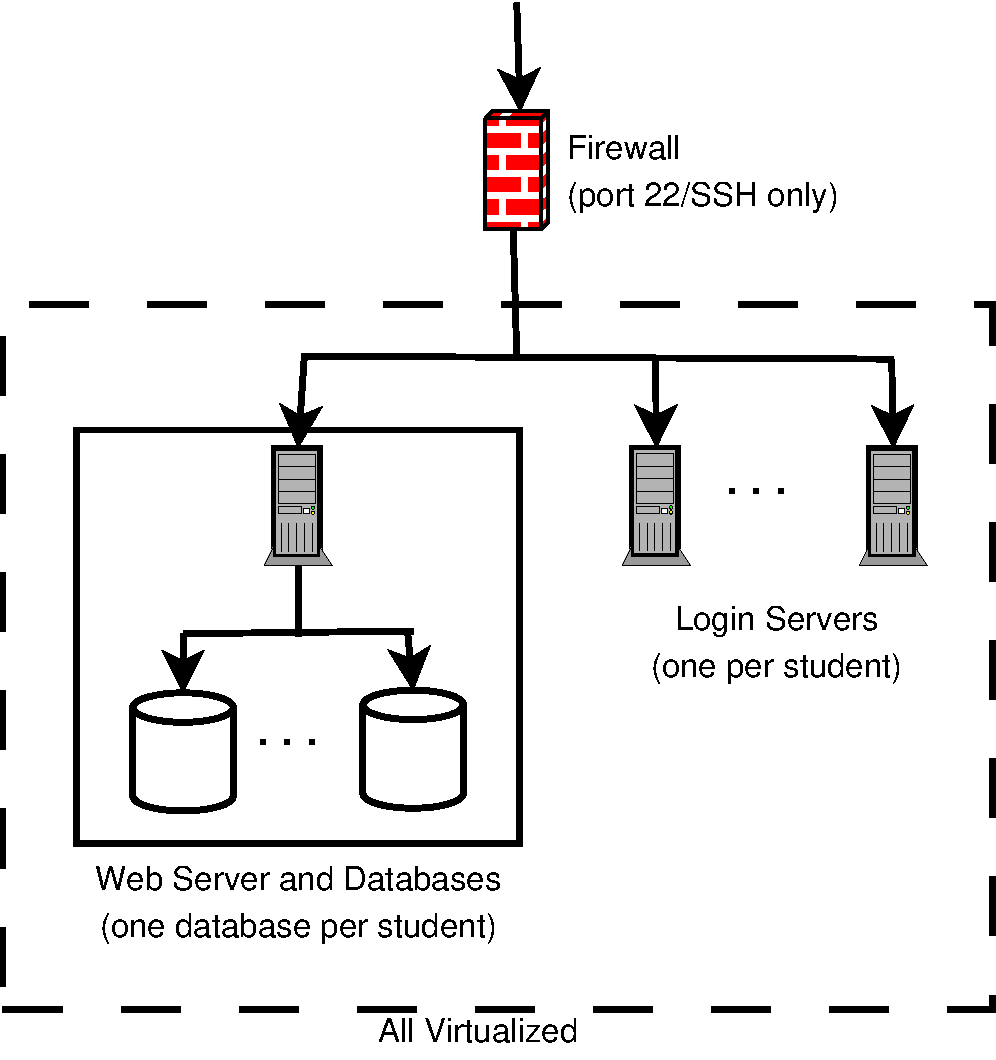
\includegraphics[width=3in]{blunderarch}
\caption{Blunderdome network architecture}
\label{fig:blunderarch}
\end{figure}

\begin{table}
\centering
\begin{tabular}{r|p{1.25in}|p{1.35in}|p{1.75in}}
Stage & Precondition	&	Attack	&	Postcondition \\ \hline \hline
1 & \raggedright Given weak SSH public key
	& \raggedright Find private key &  Login server user access \\ \hline
2 & \raggedright User-level access & \raggedright \texttt{vmsplice} privilege escalation 
	& Root on login server; web server credentials \\ \hline
3 & \raggedright Web application access & \raggedright SQL injection & Altered grade
\end{tabular}
\caption{Stages of the Blunderdome attack}
\label{table:blundertasks}
\end{table}
\TUsubsection{RFID Denial of Sleep}
\label{sec:bg:rfid}
The second case study is a denial of service attack
on the ISO 18000-7 RFID tag inventory system similar to those used by the United States
Department of Defense for shipping tracking and the Department of Energy for tracking spent
fuel containers~\cite{chen2009radiofrequency}. The attack
is similar to the ones described by Buennemeyer, \emph{et al.}~\cite{buennemeyer2006battery},
and is of a newly distinguished class of attacks sometimes termed \emph{denial
of sleep attacks}~\cite{brownfield2005wireless}~\cite{raymond2009effects}.

These ISO 18000-7 RFID tags are active and battery powered; they are used for inventory and
shipment tracking. In particular, they are used by the Department of Energy to monitor
the location and seal status of
radioactive material containers, greatly reducing workers' radiation exposure. 
The batteries on the tags should last as long as
possible in order to limit radiation exposure to maintenance workers, and
the loss of power to these devices has safety consequences.
An energy draining attack to deplete the tags' batteries could significantly
speed this loss of power.

The ISO 18000-7 tags have two modes: an active mode, and a sleep mode in which their
power consumption is significantly reduced. The active mode has a 30 second timeout,
which causes them to sleep unless the timer is reset by a valid
command from the reader or a wake-up signal. In sleep mode, the tags only respond to a
wake-up command, which causes them to enter active mode.
A denial of sleep attack occurs when the tag is not permitted to enter sleep mode or is
awoken more frequently than normal.

This attack can be realized in two ways. The first is for a second, rogue 
RFID reader to be placed by the attacker within range of active tags. The
second is for the attacker to compromise an existing reader by hacking into a computer
system connected to it via a network.

Hybrid automata serve to represent the behavior of the devices themselves quite well.
Fig.~\ref{fig:readerha} represents the reader (legitimate or rogue), which does nothing but 
transmit commands and
wake-up signals, which can come at any time with no restrictions. Under
ordinary occasional operating conditions this might take place over the course 
of as many as ten years before the batteries in the tags are 
drained~\cite{chen2009radiofrequency}.

Fig.~\ref{fig:tagha} depicts a model of a tag. For simplicity, it is shown as starting in
the active mode. It has two state variables: $c$, which represents the active mode timeout
clock, and $B$ represents the capacity of the battery. In active mode, the battery drains at
a rate of -50 per second, a rate chosen arbitrarily for illustrative purposes only. In sleep mode,
the battery drains at a rate of -1 per second. No restrictions are placed on the starting condition
of the battery. The two automata are composed using two shared actions: \emph{WakeUp} and \emph{Command}, which
synchronize the switches they decorate between the automata.

\begin{figure}
\centering
\begin{dot2tex}[options=-t raw --autosize]
digraph G {
    rankdir=LR;
    idle [shape=circle, texlbl= "Reading"];    
	idle -> idle [label="Command"];
	idle -> idle [label="WakeUp"];
}
\end{dot2tex}
\caption{Hybrid automaton model of the RFID reader}
\label{fig:readerha}
\end{figure}

\begin{figure}
\centering
\begin{dot2tex}[options=-t raw --autosize]
digraph G {
    rankdir=TD;
    awake [shape=circle, texlbl= \
    "$ \begin{matrix} \text{Awake} \\ \
    \dot{c}_{\lambda \mu} = -1 \wedge \dot{B}=-50 \\ \
    c>0 \wedge B>0 \end{matrix} $"];
    
    asleep [shape=circle, texlbl= \
    "$ \begin{matrix} \text{Asleep} \\ \
    \dot{c} = 1 \wedge \dot{B} = -1 \\ \
    B>0  \end{matrix}$"];
    
    dead [shape=circle, texlbl= \
    "$ \begin{matrix} \text{Dead} \\ \
    \dot{c} = 0 \wedge \dot{B} = 0 \\ \
    B=0  \end{matrix}$"];
	
	init [shape=none, label=""];
	
	init -> awake [label= " " \
    texlbl="$\begin{matrix} c=30 \
    \end{matrix}$"];
	
    awake -> awake [label= " " \
    texlbl="$\begin{matrix} \text{Command} \\ \
    c := 30 \
    \end{matrix}$"];
	
	awake -> awake [label= " " \
    texlbl="$\begin{matrix} \text{WakeUp} \\ \
    c := 30 \
    \end{matrix}$"];
	
	awake -> asleep [label= " " \
    texlbl="$\begin{matrix} \text{Timeout} \\ \
	c=0 \
    \end{matrix}$"];
	
	awake -> dead [label= " " \
    texlbl="$\begin{matrix} \text{Die} \\ \
	B=0 \
    \end{matrix}$"];
	
	asleep -> asleep [label= " " \
    texlbl="$\begin{matrix} \text{Command} \
    \end{matrix}$"];
	
	asleep -> awake [label= " " \
    texlbl="$\begin{matrix} \text{WakeUp} \\ \
    c := 30 \
    \end{matrix}$"];
    
	asleep -> dead [label= " " \
    texlbl="$\begin{matrix} \text{Die} \\ \
	B=0 \
    \end{matrix}$"];
    
	dead -> dead [label= " " \
    texlbl="$\begin{matrix} \text{Command} \
    \end{matrix}$"];
	
	dead -> dead [label= " " \
    texlbl="$\begin{matrix} \text{WakeUp} \
    \end{matrix}$"];
	
}
\end{dot2tex}
\caption{Hybrid automaton model of the case study active RFID tags}
\label{fig:tagha}
\end{figure}
\TUchapter{Attack Graph Generation}
\TUsection{Introduction}
Attack graph generation requires a variety of tradeoffs in terms of performance,
storage, time, expressiveness, and comprehensiveness of output. Development and
improvement of the generation methodology is a research area all to itself, one
that is not the goal of this thesis. This work is concerned with generation only
in terms of building an effective research platform from which hybrid systems
modeling can proceed.

Nevertheless, there is a dearth of straightforward presentations of attack 
graph generation algorithms, optimized for performance or not, in the 
literature. As a result, this chapter contributes a detailed treatment of the
generation algorithm used in this work. Of course, as a main goal of this
thesis is to expand on the formalism, the process evolves throughout this
work. As expansions are made, effort is given to note the changes to the
generation algorithm. Furthermore, the algorithm presented here lags behind the
state of the art in attack graph generation performance and represents a
contribution only in its explicitness.
\TUsection{Generation Algorithm and Pseudocode}
\TUsubsection{Description}
Attack graph generation proceeds in the following stages. The input to this
process is a network model specification (assets and initial fact base),
exploit pattern specification, and maximum allowed depth (actually maximum
allowed shortest path from starting state) of the constructed attack graph.

In sections where it is applicable, pseudocode is provided. As the reference
implementation is written in Python, this pseudocode uses some common Python
idioms, such as a heavy reliance upon maps (dictionaries).
\TUsubsection{Network model parsing}
The specification of the network model in the attack graph language is
parsed into a set of assets and a set of facts (the fact base). 

For the purposes
of this section, consider network state facts to be represented as ordered
tuples: for qualities, \texttt{('quality', asset, quality name, quality value)};
and for topologies, \texttt{('topology', source asset, destination asset,
topology name)}. These are stored in per-state unordered collections without duplicates
(sets) usually denoted \texttt{factbase}.

An example network model (also called network state) data model is shown in
Fig.~\ref{fig:netstate_pc}.

\begin{figure}
\begin{lstlisting}
fact-tuple = ('quality', asset, name, value) or
           = ('topology', source, dest, name)

type network_state:
    assets : set of strings;
    factbase : set of fact-tuples;
\end{lstlisting}
\caption{Network state datatype pseudocode}
\label{fig:netstate_pc}
\end{figure}

\TUsubsection{Exploit parsing}
The exploit pattern specification is parsed into a set of exploits, each
containing a set of precondition facts and a set of postcondition operations.

An example exploit data model is shown in
Fig.~\ref{fig:exploit_pc}.

\begin{figure}
\begin{lstlisting}
type exploit:
    name : string;
    params : ordered tuple of strings;
    preconditions : set of fact-tuples;
    postconditions : set of postconditions;
    
type postcondition:
    operation : 'insert' or 'delete';
    fact : fact-tuple
\end{lstlisting}
\caption{Exploit datatype pseudocode}
\label{fig:exploit_pc}
\end{figure}

\TUsubsection{Attack binding computation}
Next, the set of all possible attack bindings (recall that an attack is the
bound version of an exploit pattern) is computed and stored in memory. This
represents a list of all exploit patterns, with their parameters bound to
every possible asset permutation. That is, for each exploit pattern, a
binding must be generated for every possible asset sequence of length $n$,
where $n$ is the arity of the exploit pattern, without repetition. Pseudocode
for this stage is provided in Fig.~\ref{fig:binding_computation_pc}.

\begin{figure}
\begin{lstlisting}
def get_attack_bindings(assets, exploits): 
 attacks = [] 
 for exploit in exploits:
  param_perms = (permutations of assets with 
                    length len(exploit.params))
  for params in param_perms:
   param_bindings = map with keys=exploit.params,
                             values=params
   attacks.append( (exploit, param_bindings) )
 return attacks
\end{lstlisting}
\caption{Attack binding computation pseudocode}
\label{fig:binding_computation_pc}
\end{figure}

\TUsubsection{Attack validation}
Attack validation is a repeated process for selecting which of the exhaustively
produced attack bindings may be applied to a given network state. That is,
it comprises attack precondition processing. Two functions are described here.
One gets all valid attacks for a network state; given a network state
and a set of attack bindings, it returns the subset of those attack bindings
that may be applied to the provided network state. The second validates a
single attack binding against a network state, performing parameter binding and
checking simple set membership of the generated fact in the network state's
fact base.

Pseudocode for these two functions is provided in Fig.~\ref{fig:get_attacks_pc}.

\begin{figure}
\begin{lstlisting}
def get_attacks(network_state, attack_bindings):
 valid_attacks = []
 
 for attack in attack_bindings:
  if validate_attack(network_state.factbase, attack):
   valid_attacks.append(attack)
 return valid_attacks

def validate_attack(factbase, attack):
 # Recall: attack is of the form (exploit, binding map)
 exploit = attack[0]
 binding_dict = attack[1]
 
 for precondition in exploit.preconditions:
  if precondition.type == 'quality':
   if ('quality', binding_dict[precondition.asset], 
           precondition.name, 
           precondition.value) not in factbase:
       return False
  else if precondition.type == 'topology':
   if ('topology', binding_dict[precondition.source], 
           binding_dict[precondition.dest],
           precondition.name) not in factbase:
    return False
 return True
\end{lstlisting}
\caption{Attack validation pseudocode}
\label{fig:get_attacks_pc}
\end{figure}
\TUsubsection{Successor state computation}
Successor state computation is the second component of attack application;
it comprises postcondition processing. Its functionality is straightforward.
Given a network state and an attack binding, it first copies the network state's
component pieces. Next, it loops through the attack's
postconditions, binds parameters to assets, and removes or adds new facts
in accordance with the postcondition operation. Lastly, the network state's
components are used to construct a new network state model, the successor
state.

Pseudocode for successor state computation is provided in 
Fig.~\ref{fig:get_succstate_pc}. Note that this uses an unspecified function,
\texttt{get\_quality\_value}, whose implementation should be straightforward
with a variety of strategies. This thesis's reference implementation duplicates
network state data in a per-state map that is used only for quality lookups.
\begin{figure}
\begin{lstlisting}
def get_successor_state(network_state, attack):
 successor_assets = deep copy of network_state.assets
 successor_facts = deep copy of network_state.factbase
 
 exploit = attack[0] # (exploit, binding map)
 binding_dict = attack[1]
 
 for postcondition in exploit.postconditions:
  if postcondition.operation == 'insert':
   if postcondition.type == 'topology':
    successor_facts.insert(('topology',
        binding_dict[postcondition.source],
        binding_dict[postcondition.dest],
        postcondition.name,
        postcondition.value)
   else if postcondition.type == 'quality':
    old_value = get_quality_value(
        binding_dict[postcondition.asset], 
        postcondition.name)
    successor_facts.remove(('quality',
                            binding_dict[postcondition.asset],
                            postcondition.name,
                            old_value))
    successor_facts.insert(('quality',
                            binding_dict[postcondition.asset],
                            postcondition.name,
                            postcondition.value))
  elif postcondition.operation == 'delete':
   if postcondition.type == 'topology':
    successor_facts.insert(('topology',
                            binding_dict[postcondition.source],
                            binding_dict[postcondition.dest],
                            postcondition.name))
   elif postcondition.type == 'quality':
    old_value = get_quality_value(
        binding_dict[postcondition.asset], 
        postcondition.name)
    successor_facts.remove(('quality',
                            binding_dict[postcondition.asset],
                            postcondition.name,
                            old_value))
 return new network_state(assets=successor_assets,
                          factbase=successor_facts)
\end{lstlisting}
\caption{Successor state generation pseudocode}
\label{fig:get_succstate_pc}
\end{figure}
\TUsubsection{Attack graph generation}
Here the attack graph generation process begins in earnest. A recursive process,
the generation function operates on a collection of analysis states, a remaining
allowed depth, and an attack graph. Initially, the analysis state
list contains only the initial state, the remaining allowed depth is the maximum
depth provided at program invocation, and the attack graph is an empty graph.

Execution halts, and the attack graph is returned, if either the analysis
state list is empty, or the remaining allowed depth reaches zero.

For each state in the analysis state collection, the entire list of attacks
is checked for compatibility (by checking each of its precondition
facts for membership in the analysis state's fact base). For each suitable
attack, the analysis state is copied to a new, so-called successor state, and
the operations (insertions of facts or deletions of facts) in the attack's
postconditions are applied sequentially to the successor state. If the
successor state does not exist as a node in the attack graph, it is added. In
either case, an edge is added from the analysis state to the successor state.
A running list of all new successor states generated (that is, those that were
newly added to the attack graph) is maintained. When all possible attacks on
all analysis states have been applied, the function recurses, with the
successor states becoming the new analysis states and the remaining permitted
depth decremented by one.

Pseudocode for this process is provided in Fig.~\ref{fig:ag_generation_pc}.

\begin{figure}
\begin{lstlisting}
def generate_attack_graph(analysis_states, depth, 
                          attack_bindings,
                          attack_graph):
 if len(analysis_states) == 0 or depth == 0:
  return attack_graph
 
 # This will hold the new states added in this iteration:
 successor_states = []

 # For each state to be processed for successors:
 for analysis_state in analysis_states:
  if analysis_state not in attack_graph:
   attack_graph.add_node(analysis_state)

  # For each valid attack in that state:
  for attack in get_attacks(analysis_state, attack_bindings):
   successor_state = get_successor_state(analysis_state, attack,
                                         exploit_dict)
   if successor_state == analysis_state:
    continue
       
   if successor_state not in attack_graph:
    successor_states.append(successor_state)
    attack_graph.add_node(successor_state)
   
   attack_graph.add_edge(analysis_state, successor_state)
      
 return generate_attack_graph(successor_states, depth-1,
                              attack_bindings,
                              attack_graph)
\end{lstlisting}
\caption{Attack graph generation pseudocode}
\label{fig:ag_generation_pc}
\end{figure}
\TUsection{Example}
In order to aid understanding the generation process, this section demonstrates a
sample attack graph generation process using an example. The reader is warned to
avoid searching for meaning or design in the selection of these assets, qualities,
and topologies; they are intended to be illustrative only, and any relation to 
real world networks, problems, attacks, or situations is purely coincidental.
This section will use the network model specification in Fig.~\ref{fig:ill_nm}
and the exploit patterns in Fig.~\ref{fig:ill_xp}.
\begin{figure}
\begin{lstlisting}
network model = 
  assets :
    asset_1;
    asset_2;
    asset_3;

  facts :
    quality:asset_1,quality_1,value_1;
    quality:asset_2,quality_1,value_2;
    quality:asset_3,quality_1,value_1;
    topology:asset_1,asset_2,topology_1;
    topology:asset_3,asset_2,topology_1;
.
\end{lstlisting}
\caption{Illustrative example network model}
\label{fig:ill_nm}
\end{figure}

\begin{figure}
\begin{lstlisting}
exploit exploit_1(asset_param_1,asset_param_2)=
  preconditions:
    quality:asset_param_1,quality_1,value_1;
    topology:asset_param_1,asset_param_2,topology_1;
  postconditions:
    delete topology:asset_param_1,asset_param_2,topology_1;
    insert topology:asset_param_2,asset_param_1,topology_1;
.

exploit exploit_2(asset_param_1,asset_param_2)=
  preconditions:
    quality:asset_param_1,quality_1,value_2;
    topology:asset_param_1,asset_param_2,topology_1;
  postconditions:
    insert quality:asset_param_2,quality_1,value_2;
.
\end{lstlisting}
\caption{Illustrative example exploit patterns}
\label{fig:ill_xp}
\end{figure}

Fig.~\ref{fig:ill_topology_0} represents the initial network state 
(denoted State 0) specified
in this example. Note that Fig.~\ref{fig:ill_topology_0} is \emph{not} an attack
graph, merely a convenient graph based representation of the example network
in use here. Each node represents an asset in the network state; it is labeled
first with the state number (in this case 0) and the asset name, then with a
listing of its qualities (in this case, there is only one).
Likewise, the edges that represent topologies
are labeled with the topology name they represent.

\begin{figure}
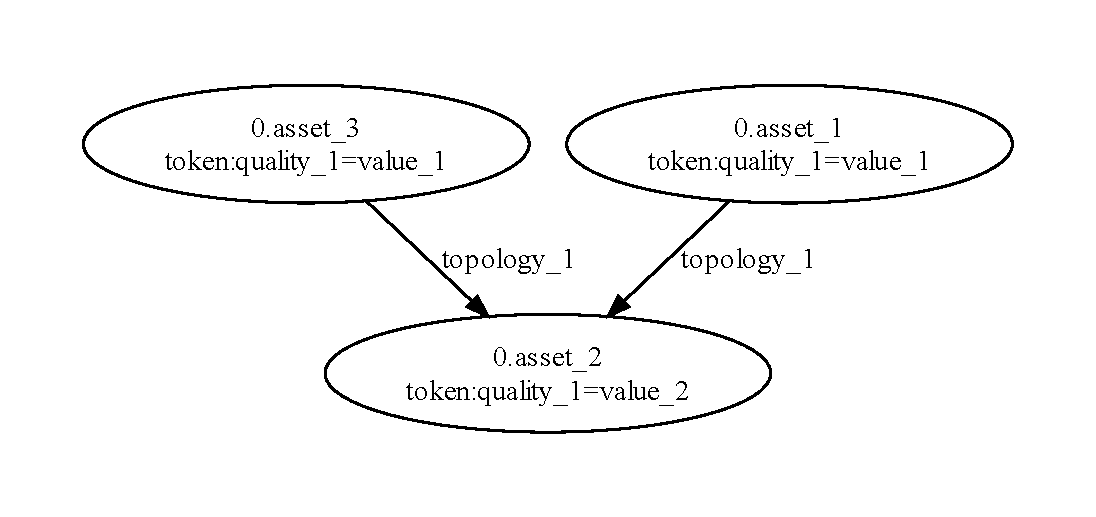
\includegraphics[width=4in]{ag_illustrative_simple/nm_state0}
\caption{State 0 of the illustrative discrete example}
\label{fig:ill_topology_0}
\end{figure}

Execution of the generation process begins by specifying a maximum ``depth''
of generation, which will be 2 for the purposes of this exercise, and by creating
an initial list of states for analysis, which contains only State 0.

Generation proceeds by examining each analysis state, in this case only State 0.
First, the generation function creates a list of all valid
attacks on State 0. Two such bindings are permitted: \texttt{exploit\_1 (asset\_1, asset\_2)},
and \texttt{exploit\_1 (asset\_3, asset\_2)}. Both bindings result in new states:
the first in State 1 (Fig.~\ref{fig:ill_topology_1}), and the second in State 2
(Fig.~\ref{fig:ill_topology_2}). Edges are added from State 0 to each as they are
generated. The current state of the attack graph is illustrated in 
Fig.~\ref{fig:ill_ag_depth1}. Both of these states are added to the
successor state list.

\begin{figure}
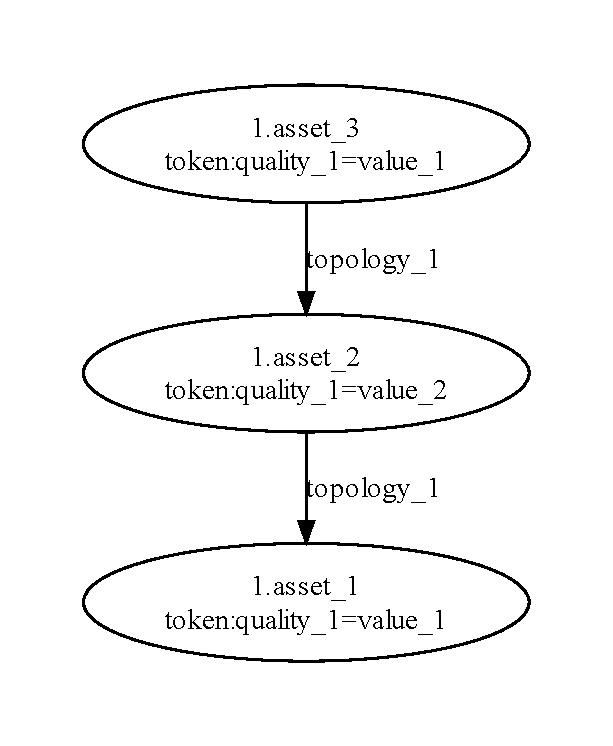
\includegraphics[width=4in]{ag_illustrative_simple/nm_state1}
\caption{State 1 of the illustrative discrete example}
\label{fig:ill_topology_1}
\end{figure}

\begin{figure}
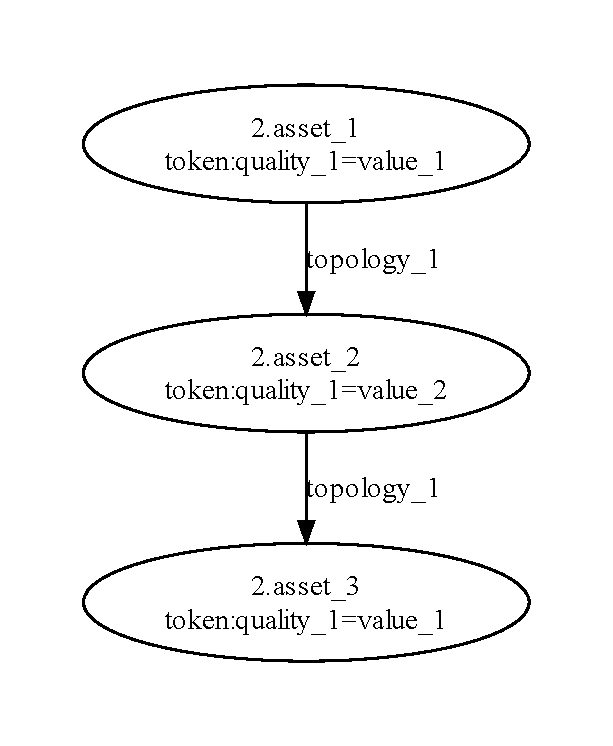
\includegraphics[width=4in]{ag_illustrative_simple/nm_state2}
\caption{State 2 of the illustrative discrete example}
\label{fig:ill_topology_2}
\end{figure}

\begin{figure}
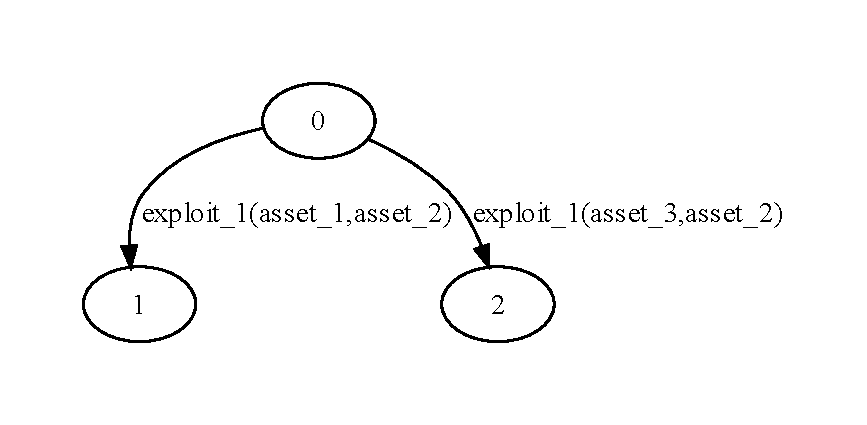
\includegraphics[width=4in]{ag_illustrative_simple/ag_depth1}
\caption{Attack graph after first iteration}
\label{fig:ill_ag_depth1}
\end{figure}

Remaining depth is reduced to 1, the successor state list becomes the
analysis state list, and generation proceeds again. In this case, the
analysis states are State 1 and State 2. Analysis begins with State 1. 
Two attacks are possible: \texttt{exploit\_1 (asset\_3, asset\_2)} and
\texttt{exploit\_2 (asset\_2, asset\_1)}. Both create new states, with the
former generating State 3 (Fig.~\ref{fig:ill_topology_3}) and the latter
generating State 4 (Fig.~\ref{fig:ill_topology_4}). Both of these are new
states, and they are added to the attack graph with the appropriate edges, as
well as to the successor state list.

\begin{figure}
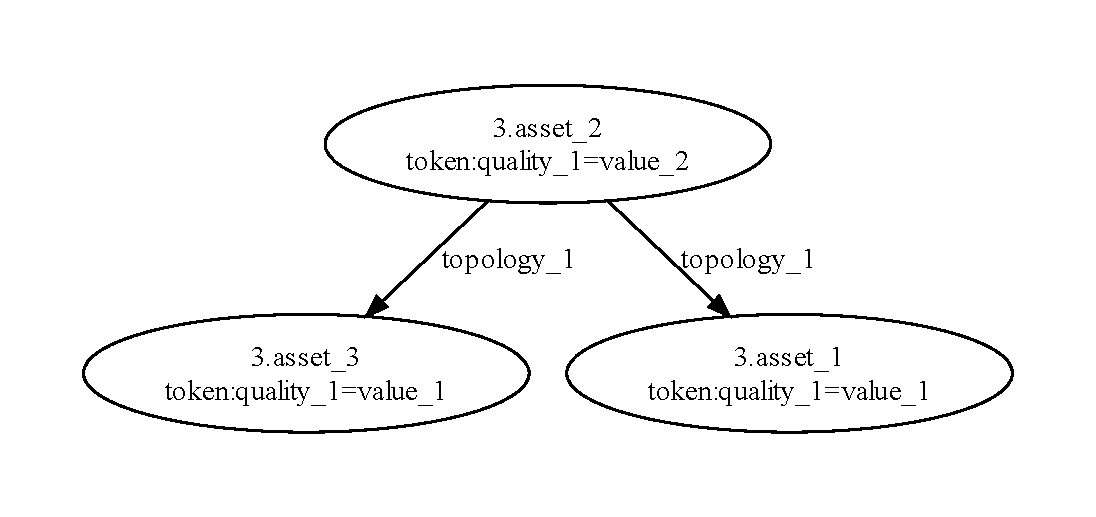
\includegraphics[width=4in]{ag_illustrative_simple/nm_state3}
\caption{State 3 of the illustrative discrete example}
\label{fig:ill_topology_3}
\end{figure}

\begin{figure}
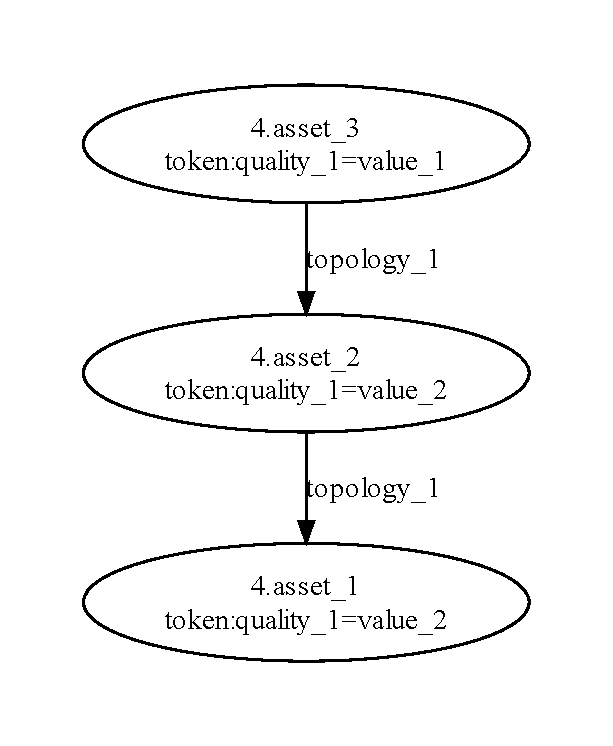
\includegraphics[width=4in]{ag_illustrative_simple/nm_state4}
\caption{State 4 of the illustrative discrete example}
\label{fig:ill_topology_4}
\end{figure}

Generation continues by addressing State 2. In State 2, two possible attacks
are returned: \texttt{exploit\_1} on \texttt{(asset\_1, asset\_2)} and 
\texttt{exploit\_2} on \texttt{(asset\_2, asset\_3)}. The first attack generates State 3,
an existing state. Since that state is already in the attack graph, it is
not added to the successor state list or to the attack graph again; instead,
only an edge is drawn. The second attack generates State 5 
(Fig.~\ref{fig:ill_topology_5}), which is new and is added to the attack graph
and the successor state list.

\begin{figure}
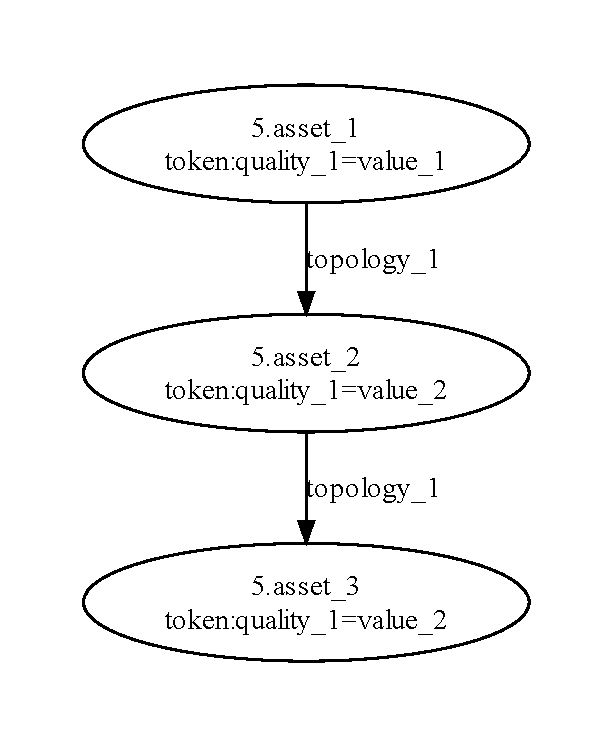
\includegraphics[width=4in]{ag_illustrative_simple/nm_state5}
\caption{State 5 of the illustrative discrete example}
\label{fig:ill_topology_5}
\end{figure}

For the next invocation, the successor state list becomes the analysis state
list, and the depth is reduced to 0.  Although there are more successor states,
the depth limit has been reached. Therefore, generation halts. The final product
attack graph is illustrated in Fig.~\ref{fig:ill_ag_depth2}. Incidentally, if
execution had been allowed to continue until there were no more successor states,
the generated attack graph would be the one in Fig.~\ref{fig:ill_ag_depth5}.

\begin{figure}
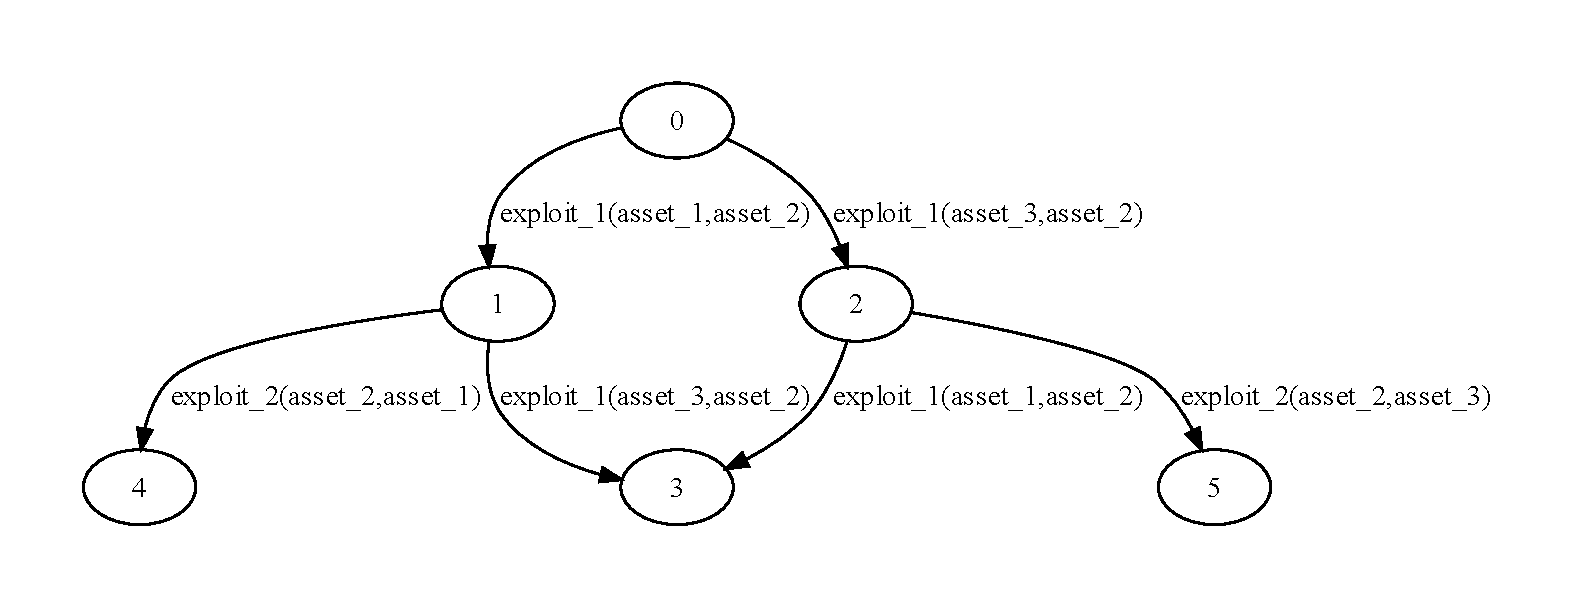
\includegraphics[width=4in]{ag_illustrative_simple/ag_depth2}
\caption{Attack graph after first iteration}
\label{fig:ill_ag_depth2}
\end{figure}

\begin{figure}
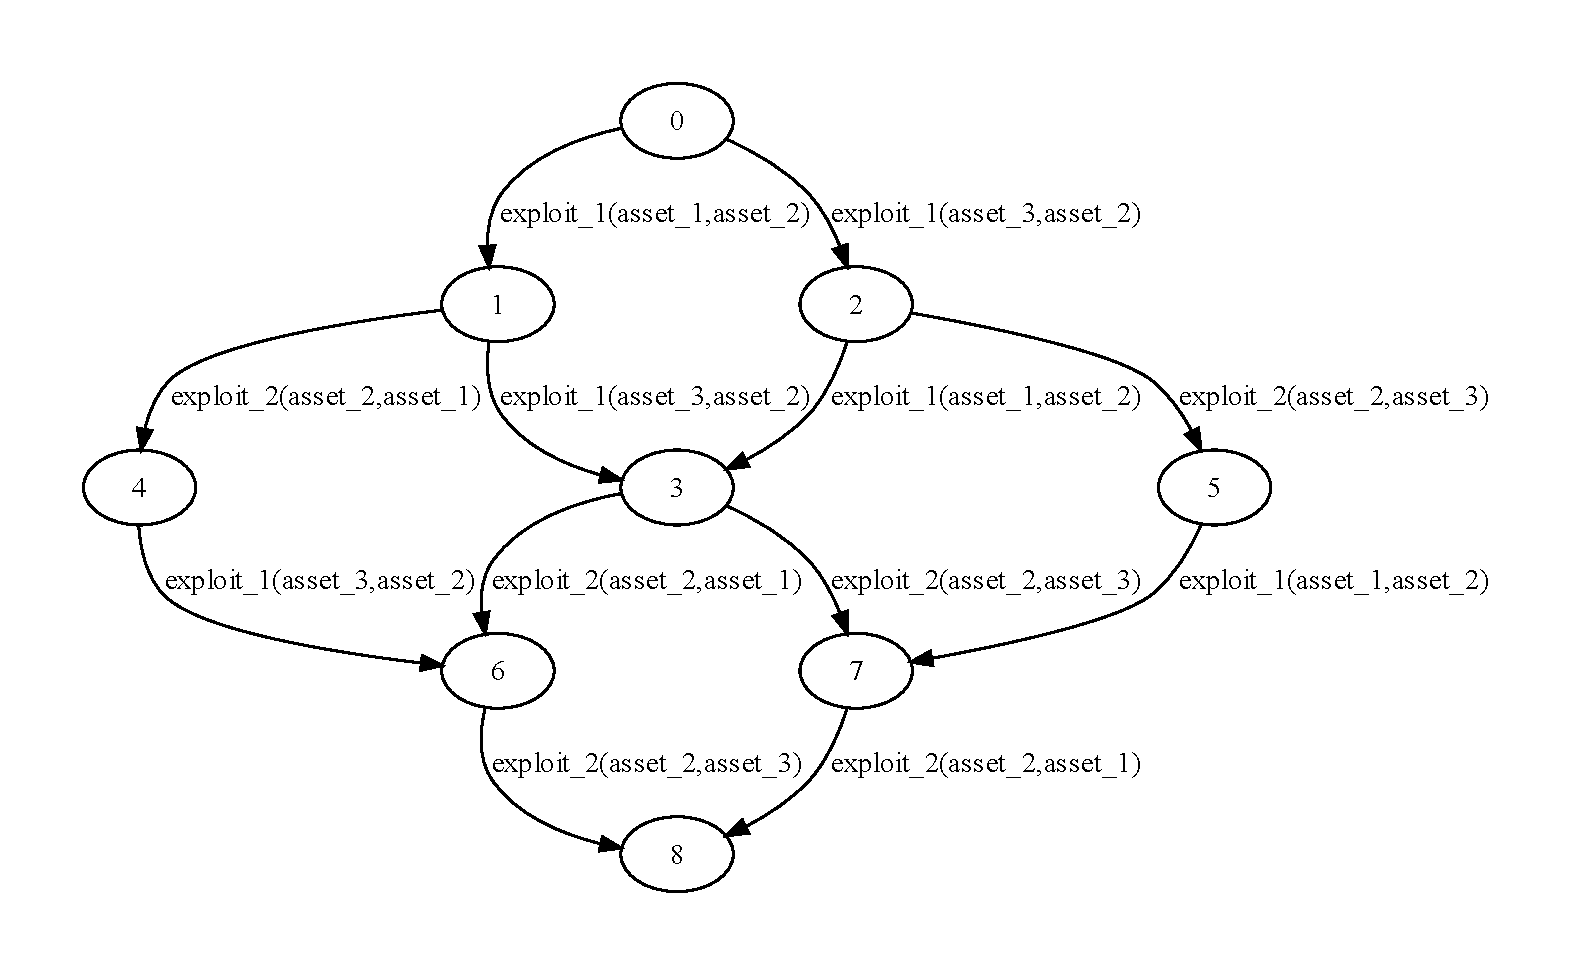
\includegraphics[width=4in]{ag_illustrative_simple/ag_depth5}
\caption{Complete illustrative attack graph}
\label{fig:ill_ag_depth5}
\end{figure}

This concludes the description of the basic attack graph modeling framework 
employed at 
the University of Tulsa. The chapters following this one are devoted to
this framework's expansion and analysis.
\TUchapter{Discrete Extensions}
\TUsection{Introduction}
For various reasons, the adaptation of the attack graph formalism described in
the preceding chapter for hybrid purposes depends upon the addition of a number
of entirely discrete elements. Their inclusion produces a transitional
attack graph formalism that is not yet appropriate for hybrid modeling but that
contains a number of enhancements suitable for discrete system modeling.

This chapter introduces these enhancements, which include a working lexicon of
standard terms for topologies and qualities based upon the Common Vulnerability
Enumeration and National Vulnerability Database; some syntactic
changes to ease the modeling of information systems; a scheme for integrating with
the Common Platform Enumeration; and some state predicate analysis tools.

\TUsection{Working Lexicon}
\TUsubsection{Introduction}
Because of the unrestricted nature of the terms available to a modeler
in this version of the attack graph framework, in order to proceed systematically
some conventions must be established in the use of terms. This thesis recommends
a set of conventions designed to ease the goal of automated exploit pattern extraction
from the National Vulnerability Database (NVD) maintained by the 
National Institute of Standards and Technology (NIST), which among other roles
indexes MITRE's Common Vulnerability Enumeration (CVE). ``NVD includes 
databases of security checklists, security related software flaws, 
misconfigurations, product names, and impact metrics''~\cite{nvdhome}.
\TUsubsection{National Vulnerability Database}
Several concepts are used across the NVD's index of vulnerabilities; they
strongly inform the working lexicon employed in this thesis and include
a vulnerability's access vector and impact type.
\TUsubsubsection{Access vector}
The access vector of a vulnerability on NVD refers to the logical location from
which the attacker may launch the attack. The possible attack vectors according
to the National Vulnerability Database are as follows.
\begin{description}
\item[Local] The vulnerability is exploitable through physical or local account access
    to the device on which the vulnerability resides.
\item[Adjacent Network] The vulnerability is exploitable through access to a network
    that is adjacent to the vulnerable host; that is, the attacker must be in the same
    broadcast domain or collision domain (e.g. the same network segment or VLAN).
\item[Network] No local or adjacent access is required to exploit the vulnerability;
    in other words, it is exploitable over the Internet.
\end{description}
\TUsubsubsection{Impact Type}
The vulnerability's impact type on NVD places the effects of the vulnerability's
exploitation on the target into one of the following categories.
, and another for some other type of privileged access.
\begin{description}
\item[Confidentiality] Confidentiality impacts allow the unauthorized disclosure 
    of information (corresponding to STRIDE's ``information disclosure'')
\item[Integrity] Allows modification of data (corresponding to STRIDE's ``tampering'')
\item[Availability] Availability impacts correspond to disruptions of service (STRIDE's
    ``denial of service'')
\item[Security Protection] The security protection category refers to the effects
    of exploits that provide unauthorized access to the target. This may be either
    general system access or application access. The security protection category
    corresponds roughly to STRIDE's ``elevation of privileges'' and also partly encompasses
    ``spoofing identity''. It has three subcategories:
    \begin{description}
    \item[User access] This subcategory refers to the attacker's gaining user level access
        to the operating system.
    \item[Administrative access] This subcategory refers to the attacker's gaining root level
        access to the operating system.
    \item[Other access] This subcategory refers to any other type of privileged access on
        the target.
    \end{description}
\end{description}
\TUsubsection{Topologies}
Introduction of actual terms begins with topologies, but first a note about the modeling
of adversaries is needed. 

Two approaches are possible for modeling the attacker. The first
is to design the network model so that it is, in a way, from the attacker's perspective.
In this scheme, henceforth the \emph{first person} strategy, the attacker is treated as
implicit, and its access and connections are considered properties of the system itself.
The adversary's access level to a server, for instance, would be modeled as a quality of
that server asset.

In the second approach, henceforth the \emph{third person} strategy, the attacker is
modeled as a first class part of the system: as an asset. Its properties, connections,
and access levels are modeled as qualities and topologies of the adversary asset.
This strategy, which is the one employed primarily in this thesis, can model multiple
adversaries. Aside from that difference, they are roughly equivalent and a matter
of taste on behalf of the modeler and analyst. This section's terminology, however,
assumes the third person model.

Two types of topology terms are introduced in this section: connection and access. These
correspond directly to the two NVD concepts introduced in the previous section.
\TUsubsubsection{Connection Topologies}
Connection topologies refer to how two assets are connected, over the network or otherwise.
They may be local, adjacent, or network connected. These connection topologies begin with
the word \texttt{connected}, followed by an underscore, then one of the three connection
types: \texttt{local}, \texttt{adjacent}, or \texttt{network}. For local and adjacent
connections, this is all that is necessary. 

For network connections it is
necessary to specify the available protocols individually. These are done by appending another
underscore, then the lower case version of the standard abbreviation for the protocol
(e.g. \texttt{connected\_network\_http} for web or \texttt{connected\_network\_ssh} for
secure shell).

Connections are one-way: the source of the connection topology is considered to be the
``client'' in the relationship, and the destination of the connection is considered
the ``server'', where such distinctions are meaningful.
\TUsubsubsection{Access Topologies}
Access topologies refer to trust relationships and distinguish what kind of access one
asset (possibly a program, individual, attacker, user, or other security principal) has
to another. Much like the subcategories of the Security Protection impact type,
there are three basic types of access topology (plus the lack of a topology, which
signifies a lack of any noteworthy trust or access relationship): user access,
root access, and other access.

They are named using the word \texttt{access}, followed by an underscore, followed
by the lowercase name of the access type, then, if the access type is \texttt{other},
an optional underscore delimited description of the access type (perhaps the name
of the application whose access level is in question). Examples include
\texttt{access\_user}, \texttt{access\_root}, \texttt{access\_other\_apache}, or
\texttt{access\_other\_vsftpd}.
\TUsubsection{Qualities}
Although qualities are used in a more \emph{ad hoc} fashion to describe entity-specific
asset properties, there is still a role for a few standard quality structures in the
lexicon, namely a simple ``status'' type of property to be used in determining
whether an asset is enabled or disabled.
\TUsubsubsection{Status}
The status property is simple but powerful. Each asset that represents a host has a
quality named \texttt{status}. It may take the value \texttt{up} or \texttt{down}.
This allows exploits against or involving the host in question to require that it
be online as a precondition, and it provides a simple mechanism of action for
denial of service attacks to be modeled -- they simply have the postcondition of
a \texttt{status = down} quality fact.

Later in this chapter, a simple preprocessor combined with a dash of syntactic sugar
is introduced to automate most of the status modeling process across both exploits
and the network model.

\TUsection{Syntactic Sugar}
\TUsubsection{Directional Topologies}
This section introduces a new notation for specification of topologies. As it
is common to model bidirectional topologies, an additional convenience syntax
is now permitted to specify the directionality of a topology. As before, 
topologies are specified by the word~\texttt{topology}, followed by a colon, 
followed by the names of the assets in question; however, in the new syntax,
they are separated not by a comma but by a directionality symbol:~\texttt{->} to 
represent a one-way topology from the left asset to the right asset,
or~\texttt{<->} to represent a two-way topology. To promote readability, there
is no~\texttt{<-} directionality permitted.

Furthermore, the model has no innate distinction between one-way and two-way
topologies except the \texttt{<->} shorthand for specifying symmetric topologies.
That is to say, a bidirectional topology fact is actually implemented as
two unidirectional topology facts. Therefore, for example, if a bidirectional
topology exists in the fact base, one of its component directional topologies may
be removed by the realization of an exploit without affecting its reverse.
\TUsubsection{Value Assignment}
In preparation for the introduction of real-valued facts, the existing discrete
type of qualities, henceforth called ``token valued'', are given a special
assignment operator. Simply put, token values are assigned with the~\texttt{=}
operator and tested with the~\texttt{=} and~\texttt{!=} operators. This
enables a robust distinction between assignment operators and relational
operators.

Additionally, \texttt{delete} operations in postconditions take only a quality
name, with no value required (eliminating the confusing possibility of a
command to \texttt{delete quality:a,q!=5}, one of several deletion commands
that has little meaning).
\TUsubsection{Host Declaration and Status Proprocessing}
To support the use of status properties of host assets, a set of shorthand
syntax is now provided for denoting which assets represent hosts. In practice,
this has been observed to be the majority of modeled assets, so the shorthand
is highly convenient for modelers. Host denotation and status processing is 
done in two places: in the declaration of assets, and in the parameter list of 
exploits.

In the asset list declaration, up hosts are denoted by prefixing their name with
the symbol~\texttt{@}, a signal to the host preprocessor to automatically add
the \texttt{quality:hostname,status=up} fact; and down hosts are denoted with
the~\texttt{!@} symbol, automatically adding the down host quality fact.

Similarly, in exploit parameter lists, asset parameters that must have the
up status precondition are declared by prefixing their names with the up host 
symbol~\texttt{@}; likewise with the down symbol~\texttt{!@}. If no host
status preconditions are required, no symbol is needed. The host status
preprocessor automatically adds the required preconditions; if a host status
postcondition is necessary, for example in the case of a denial of service
attack bringing a host offline, the status property must be manually specified;
this is not a significant burden, as this case arises considerably less
frequently.
\TUsubsection{Global and grouped exploits}
For a variety of modeling tasks, it is convenient to cause an exploit to be
fired on all possible bindings simultaneously or to synchronize two exploits'
firing with one another. Two optional keywords are now permitted at the beginning
of the exploit header for this purpose: \texttt{global} and \texttt{group()}.
The \texttt{group} keyword takes a single argument.

Their semantic behavior
is as follows. When a global exploit is fired on one binding of assets, it will
also be fired on all other assets for which a valid binding exists, and the
corresponding state transition will be considered a single edge on the attack
graph. When a group exploit is fired on a binding of assets, all other exploits
denoted with the group keyword and the same group argument will also attempt
to fire on the same asset binding. Obviously grouped exploits require the same
number of parameters.

Two \emph{caveats} are required with global and grouped exploits. The first
is that a group may not mix global and nonglobal exploits. If mixing of
nonglobals and globals were permitted within a single group, the result would
be behavior that is compatible with neither the concept of a group or the
concept of a global (a group requires that each single attack binding be made
to all exploits within the group, whereas a global requires every possible
attack binding be made simultaneously).

The second warning is that no consistency checking is specified. That is,
preconditions are checked against a predecessor state, then postconditions
are applied in arbitrary order. This means that if multiple attacks in a group
modify the same facts on the same assets, indeterminate behavior or race
conditions may occur. For this reason, it is advised to group exploits that
will not do this.
\TUsubsection{Platform Properties}
Platform facts are new types of facts introduced by this work. They use the
specification used by MITRE's Common Platform Enumeration (CPE), a component
of the Security Content Automation Protocol (SCAP). (TODO: CITE)
They can specify operating systems, applications, and hardware.

A CPE platform fact is simply a valid CPE URI tied to an asset. The CPE URI is
comprised of the word \texttt{cpe}, a 
colon, then a slash, then the part type (\texttt{o} for operating system, \texttt{a} for
application, or \texttt{h} for hardware), then a colon, then the CPE vendor abbreviation,
then a colon, then the CPE product abbreviation, a colon, the version, a colon, the update, a colon, 
the edition, a colon, then the language. Version is required, but the rest is optional.

For example, to specify that a host is running Adobe Reader version 8.1, a 
platform fact named \texttt{cpe:/a:adobe:reader:8.1} would be used. Platforms
are matched according to the algorithms provided in the CPE specification,
permitting blank (wildcard) fields and the prefix property.
\TUsection{Generation process changes}
These new capabilities require some adjustments to the semantic behavior of the
attack graph generation generation process. Happily, the attack graph generation
algorithm itself is unchanged, although more sophisticated fact handling,
both for precondition processing and postcondition application,
is required. This section discusses briefly these changes.
\TUsubsection{Bidirectional topologies}
The addition of bidirectional topologies introduces a new requirement for
parsing or precondition/postcondition analysis: that single bidirectional 
topology facts be decomposed into pairs
of unidirectional topologies. In the reference implementation, this is done
not in the initial parse itself but rather in the portion of fact handling that
converts the raw parsed data structure into the generator's internal fact
data structure.
\TUsubsection{Platform properties}
The new platform properties introduce another set of conditional logic to
precondition processing. Since there are no operators, precondition matching
is relatively simple syntactically; however, because of the prefix
property of its encoding and the ability to have blank ``wildcard'' fields
in the matched CPE, a matching algorithm must be used. The matching algorithm
in the reference implementation is based on the one provided in the CPE
specification. %TODO: CITE
The pseudocode for this thesis's platform fact matching functionality is
provided in Fig.~\cite{fig:cpe_match_pc}

\begin{figure}
\begin{lstlisting}
def has_platform(factbase_platformlist, platform):
 # Platform is a tuple
 for cpe in factbase_platformlist:
  if len(cpe) >= len(platform):
      ret = False
      for components in zip(cpe, platform):
       if components[0] == components[1] or platform == '':
        ret = True
       else:
        ret = False
        break
       if ret:
        return cpe # Return the matched platform
 return False
\end{lstlisting}
\caption{Platform fact matching pseudocode}
\label{fig:cpe_match_pc}
\end{figure}
\TUsubsection{Precondition matching}
On the other hand, precondition matching for quality facts must become
somewhat more complicated with the addition of the not-equal relational
operator. Merely building a fact and checking for its membership in the
factbase data structure is no longer sufficient. 

Although the not-equal relational operator \emph{could} be implemented
similarly to the equality relational operator, by building a fact from the
given name and value and checking for its exclusion from (instead of inclusion 
in) the factbase, a more advanced fact checking method is provided in order 
to ease the transition to permitting real values for qualities.

The fact base data structure is updated to include maps from quality names to
quality values in order to facilitate lookup. Although this results in an
increased storage requirement, it prevents costly lookups in the existing
factbase data structure. Fact checking, then, is done using these simple hash
table lookups and comparisons. A new specification for the network state
data structure reflecting these changes is provided in 
Fig.~\ref{fig:netstate_map_pc}.

\begin{figure}
\begin{lstlisting}
fact-tuple = ('quality', asset, name, value) or
           = ('topology', source, dest, name) or
           = ('platform', platform_part, ..., language)

type network_state:
    assets : set of strings;
    factbase : set of fact-tuples;
    qualities : map (keys=assets, vals=map(keys=quality_name,
                                           vals=quality_value))
\end{lstlisting}
\caption{Updated discrete network state datatype pseudocode}
\label{fig:netstate_map_pc}
\end{figure}

\TUsubsection{Global and grouped exploits}
The simultaneous application of global and grouped exploits is also
fairly straightforward. Postcondition processing requires only the minor change
of permitting a list of postconditions to be processed sequentially (which
really only requires the union of their postcondition facts) using the
existing postcondition application method.

Precondition processing, however, insofar as it causes the selection and
grouping of attacks that should be fed into the generation function,
each producing its own state transition, is somewhat more commplex. To permit
a reader to follow along, pseudocode is provided in 
Fig.~\ref{fig:cpe_glgr_precondition_pc}.

The reference implementation uses a two-pass algorithm over the set of
valid attacks (selected using the existing precondition processing method).
First, a pair of mappings are instanciated to store the attack data structures.
The group mapping is keyed on group names and has as values more maps, which are
themselves keyed to tuples of assets (representing bindings values) and valued
with specific attack bindings. The global mapping is keyed on exploit name
and also valued with attack bindings.

The first step is to loop through all the attacks. Attacks are placed in the
appropriate map (or maps) depending on their group (and binding) and global
configuration.

The second step is to use these maps to generate groupings of attacks, which
are to be applied by the postconditions processor in the same manner as single
attacks themselves are applied. First, groups and bindings are looped through.
A grouping is generated for each group name. If the members of the group are
from global exploits, their attacks are loaded from the global map (and
subsequently removed from the global map). Otherwise, they are added individually
from the group/binding map.

Once each exploit's attacks are added according to a particular binding, either
(if the group is nonglobal) the next binding is consulted, which begins a new
attack aggregation, or execution breaks to the next group (if the group is
global, meaning that every possible binding has already been added). Finally,
each remaining global exploit (that is, the ungrouped global attacks) is
added as its own attack grouping. The groupings are returned.
\begin{figure}
\begin{lstlisting}
    group_dict = map keyed on group name
    globl_dict = map keyed on exploit name
    
    for attack in attacks:
        group = attack.group
        globl = attack.globl
        binding = attack.binding.values # asset list

        if group:
            if group in group_dict and binding in group_dict[group]:
                group_dict[group][binding].append(attack)
            elif group in group_dict:
                group_dict[group][binding] = [attack,]
            else:
                group_dict[group] = new map{binding : [attack,]}
        if globl:
            if attack.name in globl_dict:
                globl_dict[attack.name].append(attack)
            else:
                globl_dict[attack.name] = [attack,]
    
    agg_attacks = [] # Aggregated attacks

    for group_id in group_dict:
        group_attacks = group_dict[group_id]
        for binding in group_attacks:
            agg_group = []
            group_is_global = None
            for attack in group_attacks[binding]:
                if attack.name in globl_dict: # group and global
                    agg_group += globl_dict[attack[0]]
                    remove globl_dict[attack[0]]
                    if group_is_global == False: error
                    group_is_global = True
                else: # Not global
                    if group_is_global == True: error
                    group_is_global = False
                    agg_group.add(attack)
            agg_attacks.append(agg_group)
            if group_is_global:
                # Global status already covers all bindings
                break
    for globl_attack in globl_dict: # ungrouped globals
        agg_attacks.append(list(globl_dict[globl_attack]))
\end{lstlisting}
\caption{Group and global attack selection}
\label{fig:cpe_glgr_precondition_pc}
\end{figure}
\TUsection{Examples}
\TUsubsection{Illustrative}
For completeness, this section provides the updated syntax's version of
Chapter 3's example, which is otherwise unchanged. The network model is
provided in Fig.~\ref{fig:ill_updated_nm}, and the exploit patterns are
provided in Fig.~\ref{fig:ill_updated_xp}.

\begin{figure}
\begin{lstlisting}
network model = 
  assets :
    asset_1;
    asset_2;
    asset_3;

  facts :
    quality:asset_1,quality_1=value_1;
    quality:asset_2,quality_1=value_2;
    quality:asset_3,quality_1=value_1;
    topology:asset_1->asset_2,topology_1;
    topology:asset_3->asset_2,topology_1;
.
\end{lstlisting}
\caption{Illustrative example network model in the new format}
\label{fig:ill_updated_nm}
\end{figure}

\begin{figure}
\begin{lstlisting}
exploit exploit_1(asset_param_1,asset_param_2)=
  preconditions:
    quality:asset_param_1,quality_1=value_1;
    topology:asset_param_1->asset_param_2,topology_1;
  postconditions:
    delete topology:asset_param_1->asset_param_2,topology_1;
    insert topology:asset_param_2->asset_param_1,topology_1;
.

exploit exploit_2(asset_param_1,asset_param_2)=
  preconditions:
    quality:asset_param_1,quality_1=value_2;
    topology:asset_param_1->asset_param_2,topology_1;
  postconditions:
    insert quality:asset_param_2,quality_1=value_2;
.
\end{lstlisting}
\caption{Illustrative example exploit patterns in the new format}
\label{fig:ill_updated_xp}
\end{figure}

\TUsubsection{Blunderdome}
This section presents an attack graph model of the Blunderdome exercise
described in section~\ref{sec:blunderdome}.
\TUsubsubsection{Network Model}
The network model for the Blunderdome exercise follows in a straightforward
from the network diagram (Fig.~\ref{fig:blunderarch}), including each network
element as an asset, plus an asset for the attacker. The facts include the
attacker's grade on the web server, the SSH and HTTP connection topologies,
and platform facts for the relevant applications and operating systems subject
to exploitation: OpenSSL, Linux, and the Blunderdome specific grades tracking
application (which receives a dummy CPE entry).

\begin{figure}
\begin{lstlisting}
network model = 
 assets :
  attacker;
  login_server;
  web_server;
    
 facts :
  quality:web_server,grade=F;
  topology:attacker->login_server,connected_network_ssh;
  topology:login_server->web_server,connected_network_http;
  platform:login_server,cpe:/a:openssl_project:openssl:0.9.8c-1;
  platform:login_server,cpe:/o:linux:kernel:2.6.24;
  platform:web_server,cpe:/a:isec:blundergrades;
.
\end{lstlisting}
\caption{Blunderdome network model}
\label{fig:blunder_nm}
\end{figure}

In this model there are three access topologies in play: access\_admin,
access\_user, and access\_other\_blunderdome, representing access to the 
Blunderdome web application.
\TUsubsubsection{Exploit Patterns}
The exploits in the Blunderdome exercise, provided in Fig.~\ref{fig:blunder_xp}
fall into three categories. The first is the set of straightforward CVE-based exploits
that could easily be extracted automatically from the National Vulnerability
Database. The second is the hand generated exploits like blunder\_sqli, which
has hand-generated custom behavior to modify the attacker's grade. The third
are the exploit patterns that do not necessarily represent abuse cases 
but rather state transitions due to attacker actions.

\begin{figure}
\begin{lstlisting}
exploit CVE_2008_0166_1(a, l)=
 preconditions:
  platform:l,cpe:/a:openssl_project:openssl:0.9.8c-1;
  topology:a->l,connected_network_ssh;
 postconditions:
  insert topology:a->l,access_user;
.

exploit CVE_2008_0600_1(a,l)=
 preconditions:
  topology:a->l,access_user;
  platform:l,cpe:/o:linux:kernel:2.6.24;
 postconditions:
  insert topology:a->l,access_admin;
.

exploit blunder_sqli(a,w)=
 preconditions:
  platform:w,cpe:/a:isec:blundergrades;
  topology:a->w,access_other_blunderdome;
 postconditions:
  insert quality:w,grade=A;
.

exploit ssh_http_tunnel(a,l,w)=
 preconditions:
  topology:a->l,connected_network_ssh;
  topology:a->l,access_user;
  topology:l->w,connected_network_http;
 postconditions:
  insert topology:a->w,connected_network_http;
.

exploit blunder_login(a,l,w)=
 preconditions:
  topology:a->w,connected_network_http;
  topology:a->l,access_admin;
 postconditions:
  insert topology:a->w,access_other_blunderdome;
.
\end{lstlisting}
\caption{Blunderdome exploit patterns}
\label{fig:blunder_xp}
\end{figure}

The first two exploits could be automatically generated from the CVE entries
in the NVD. The third was hand generated due to its being an internal custom 
piece of software without NVD entries and the complex behavior the exploit must
encode.

The next exploit, ssh\_http\_tunnel, represents a common idiom involved in
attack chaining: using access to one machine to create new access topologies
to adjacent machines. The last exploit, blunder\_login, represents access to
the Blunderdome credentials due to administrative access to the login
server. This could also be modeled using an additional asset representing the
credentials, but for simplicity the method with fewer assets is demonstrated.

The resulting attack graph is provided in Fig.~\ref{fig:blunder_ag}; the
graphical representation of the starting state and ending state in 
Fig.~\ref{fig:blunder_s0} and Fig.~\ref{fig:blunder_s6}.

\begin{figure}
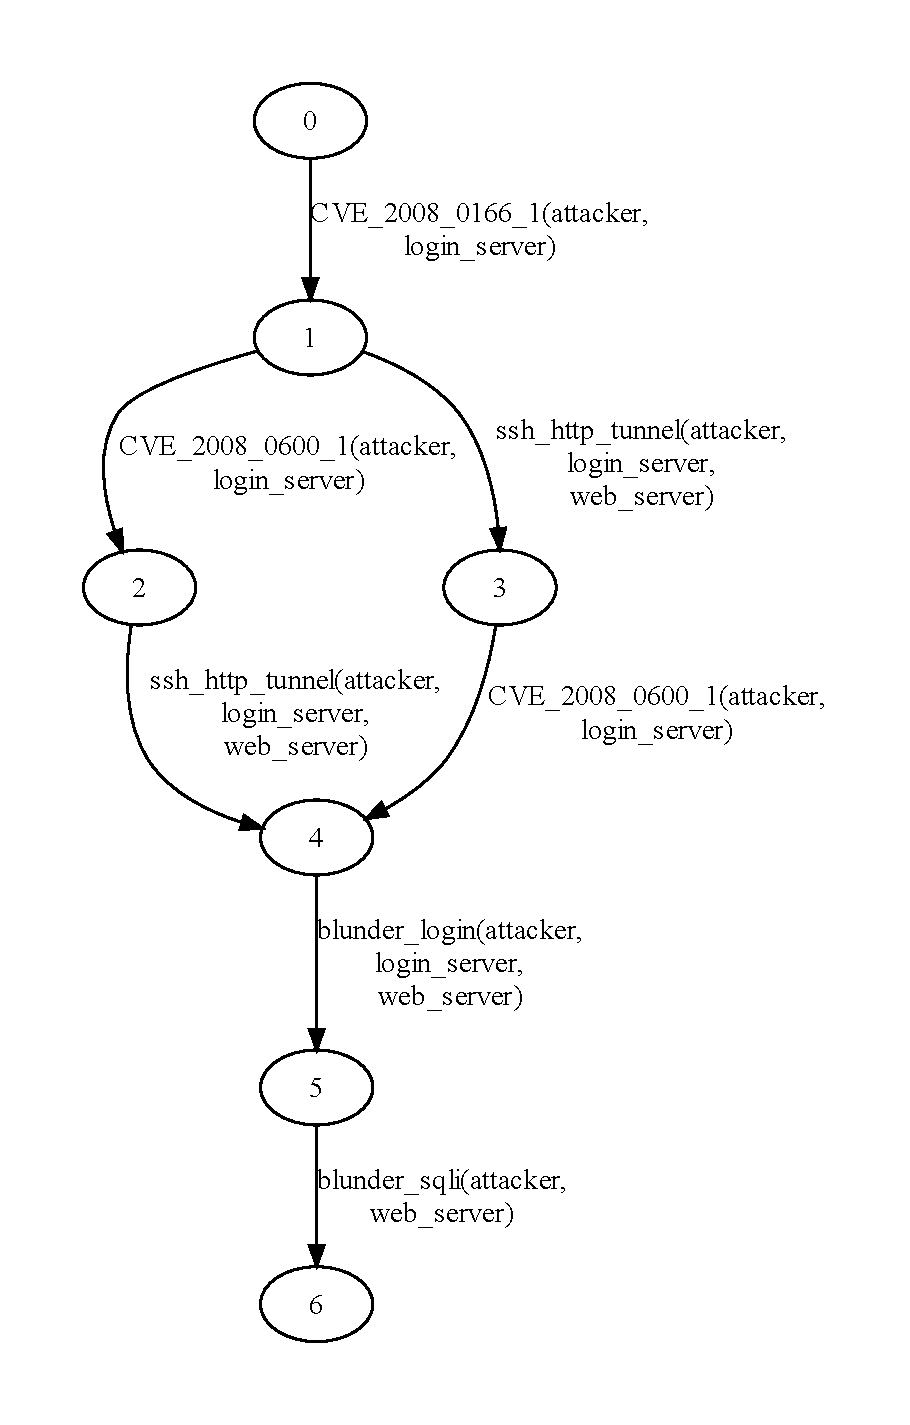
\includegraphics[width=5in]{ag_blunderdome/ag_depth5}
\caption{Blunderdome exercise attack graph}
\label{fig:blunder_ag}
\end{figure}

\begin{figure}
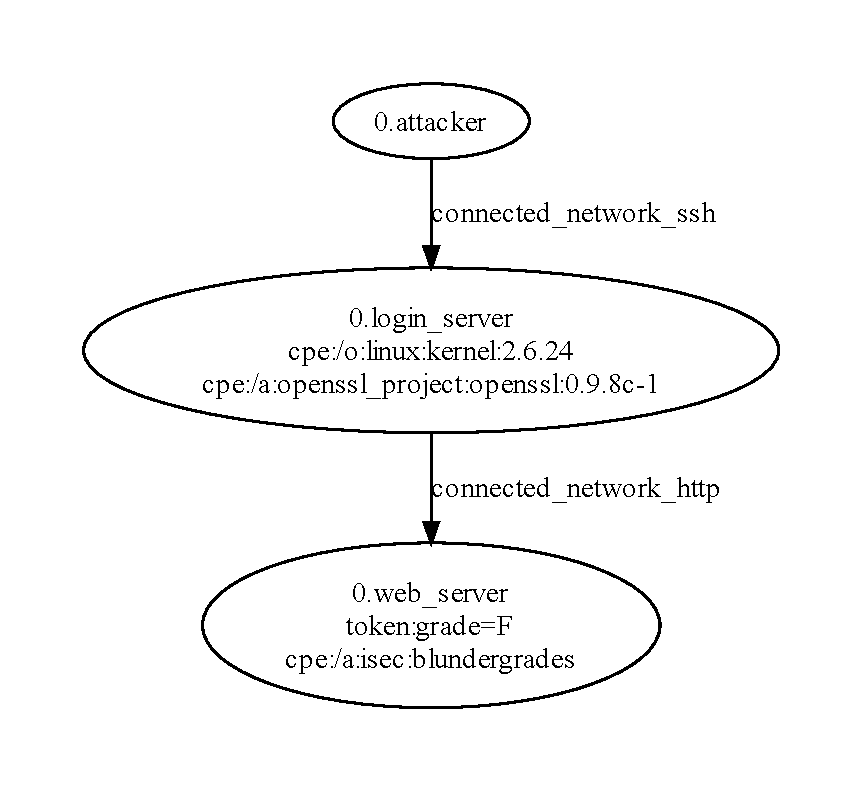
\includegraphics[width=5in]{ag_blunderdome/nm_state0}
\caption{Blunderdome exercise starting state}
\label{fig:blunder_s0}
\end{figure}

\begin{figure}
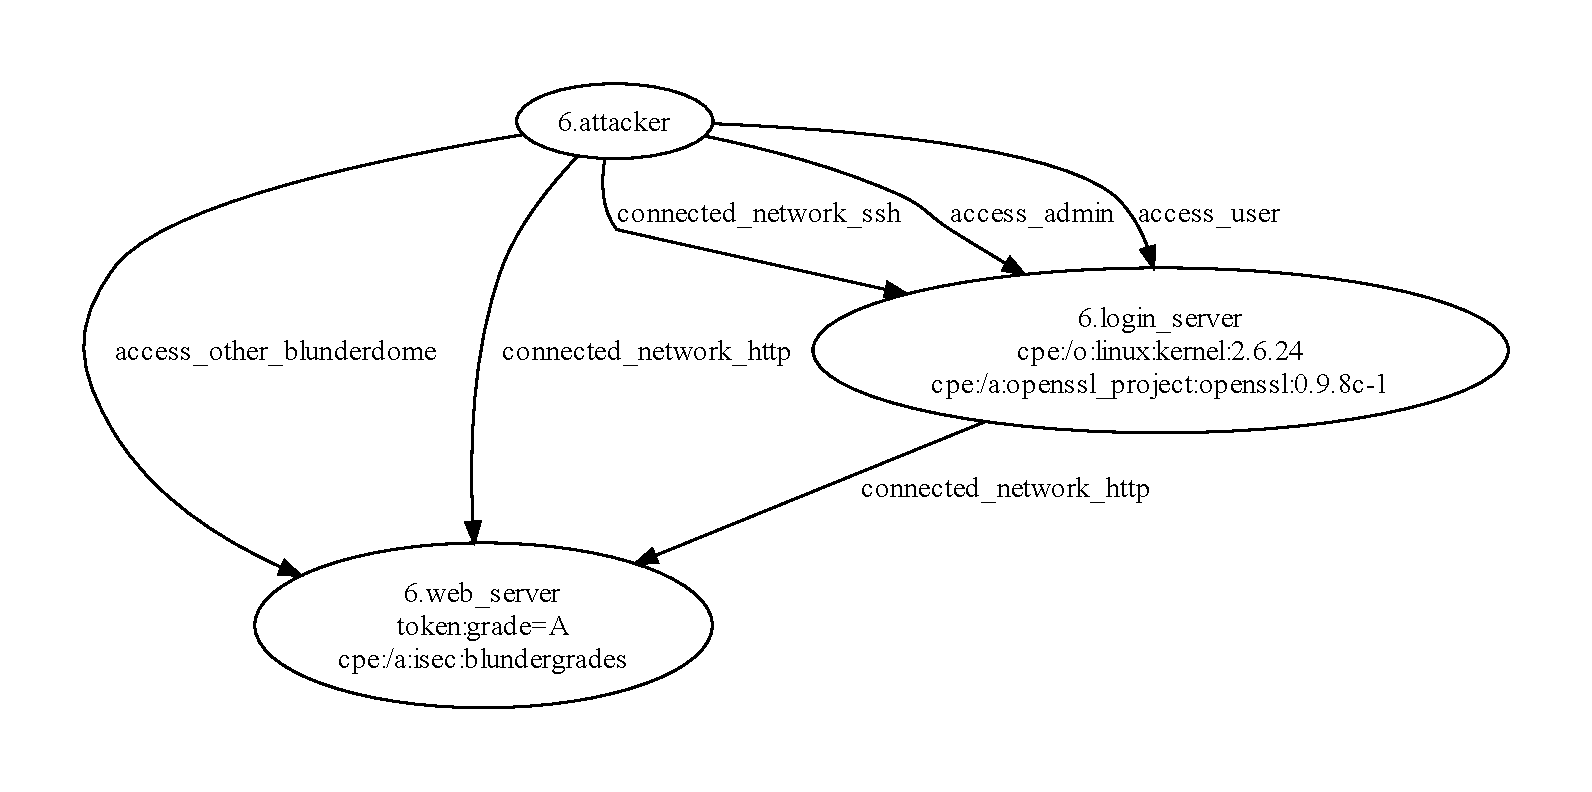
\includegraphics[width=5in]{ag_blunderdome/nm_state6}
\caption{Blunderdome exercise ending state}
\label{fig:blunder_s6}
\end{figure}

\TUchapter{Hybrid Extensions}
\TUsection{Introduction}
An objective of this thesis is to make the first known foray into the realm of
attack graphs with real-valued components. This chapter introduces the additional
modeling syntax and generation semantics required to permit real values for
qualities and topologies. Furthermore, some initial attempts at representing
the passage of time are described. 

The ultimate goal of the specification of a hybrid attack graph for cyber
physical systems modeling must be the creation of a formalism capable of
modeling a network containing both traditional information systems (as
existing attack graph incarnations can) and hybrid systems (i.e. those that
can be modeled as hybrid automata). Therefore, the ideal hybrid attack graph
should be able to define systems (assets) that have some equivalence to a
hybrid automaton.

This thesis presents two novel attack graph elements with this requirement
in mind. The first is the ability to give both qualities and topologies
real (continuous domain) values, and correspondingly to permit exploits to
test and operate on these values in the expected ways with a full selection of
real-valued relational and assignment operators. These new types of facts are 
at the heart of this new model. 

The second contribution is modeling the progression
of time; as implemented in this thesis, time progression does not require any
new syntactic elements as compared to those provided in the discrete 
enhancements in the preceding chapter; those syntactic elements, however, are
used in a novel fashion to specify the
time evolution of quality and topology values.

The remainder of this chapter is structured as follows. First, the new
syntactic elements are introduced. Second, the semantic changes that these new
elements impose upon the generation process are described. Then the current
convention for the specification of time evolution is described. Next, 
time state aggregation, an enhancement for cognitive scalability purposes,
is introduced along with its semantic changes to the generation process.
Finally, a pair of examples are provided illustrating the ability of the
hybrid attack graph not only to capture cyber physical systems, but also to
enhanc the modeling capabilities of attack graphs for traditional information
systems.
\TUsection{Definition of New Syntax}
\TUsubsection{Terminology}
First and foremost, a discussion of the new terminology involved in the
transition to hybrid attack graphs is required. This is mostly concerned with
facts, as the movement to hybrid attack graphs is mostly concerned with changes
to the fact system.

Until now, qualities have had only string type values, and
topologies have had no values at all. In this chapter, that changes. Although
there will always remain a need for these discrete valued qualities and name
only topologies, there is also a need for qualities with 
continuous, numerical values. The introduction of a second type of quality
value is somewhat less jarring, however, than that of topologies with
values.

As the hybrid attack graph introduced by this thesis is a strict superset
of the University of Tulsa style discrete attack graph, the existing style
of quality and topology facts remains valid in the new language and therefore
must be distinguished from the new type of fact in some way. The discrete
only facts, therefore, are called \emph{token valued} (or \emph{token facts},
whereas the new continuous facts are called \emph{real valued} (or \emph{real
facts}).

% Additionally, later in this chapter another class of fact is introduced: a
% rate fact, which is a special case of a real fact. Rate facts are not a new
% syntactic element but are rather specified by convention and invoked by the
% new timing capability. TODO: this isn't true; add to future work.
\TUsubsection{Operators}
At the heart of the hybrid attack graph lies the new real facts. Their
existence marks the introduction of a true type system to the attack graph
model, which must be dealt with in some fashion. Furthermore, these new real 
facts demand new real operators to deal with them.

Typing is dealt with by ensuring that the sets of both assignment and relational
operators used for token and real facts are disjoint. While token qualities are
assigned with the \texttt{=} operator, real facts (both quality and topology)
are assigned using a \texttt{:=} operator.

As for the relational operators, token facts are tested using \texttt{=} 
and \texttt{!=}. The relational operators permitted for real facts (both
quality and topology) are different: \texttt{==}, \texttt{>}, \texttt{>=},
\texttt{<=}, and \texttt{<>} (for not equal).

Finally, because a principal property of real values is their suitability for
arithmetic, a number of new operators are introduced for use in exploit
postconditions only, with their straightforward C-like meanings: \texttt{:=},
\texttt{+=}, \texttt{-=}, \texttt{*=}, and \texttt{/=}. Note that currently
these operators take only literal reals as their second operand; variables
are not permitted.
\TUsubsection{Topology values}
Due to the usefulness of permitting real valued relationships between assets,
be they physical such as distance, or IT related like latency or signal
strength, in hybrid attack graphs, real topologies may take values. The
syntax for this is identical to the existing token topology syntax, except
followed by an operator and a number.

\TUsubsection{The update operation}
Because of the semantics of binary arithmetic operators such as \texttt{+=},
the term \texttt{insert} in postcondition operations is somewhat psychologically
unsatisfactory. Therefore, it is now aliased to \texttt{update}, a semantically
identical operation. In spite of its apparent redundancy, it provides for
future expansion as well as readability.
\TUsection{Time}
A fundamental requirement of modeling hybrid systems is the progression of
time, as the most interesting and distinctive properties of physical processes
are their evolution over time. Another goal is to avoid introducing additional
special cases. To that end, this section introduces a method for handling time
using only previously introduced attack graph functionality.
\TUsubsection{Time exploits}
Exploits are not just for adversary actions anymore. Time is implemented using
a single group of global exploits, each of which increments a class of assets'
position in time depending upon its particular state. The global status
causes them to trigger on all assets simultaneously, while the grouping causes
all the time exploits to trigger in concert with each other. As before,
an important requirement is that the sets of facts affected by time exploits
be disjoint over all grouped time exploits to avoid indeterminate behavior.

A selection of time exploits is provided in Fig.~\ref{fig:illustrative_time_xp}
of time exploits that might simplistically model
a car driving away from a wall unless somehow compromised by an attacker,
who causes the car to drive toward the wall at a constant rate.

\begin{figure}
\begin{lstlisting}
network model=
    assets:
        civic;
        wall;
    facts:
        platform:civic,cpe:/h:honda:civic;
        quality:civic,compromised=true;
        quality:civic,status=up;

        platform:wall,cpe:/h::wall;

        topology:civic<->wall,distance:=50;
.
\end{lstlisting}
\caption{Car example network model}
\label{fig:illustrative_time_nm}
\end{figure}

\begin{figure}
\begin{lstlisting}
global group(time) exploit car_depart(c,w)=
    preconditions:
        platform:c,cpe:/h:honda;
        quality:c,compromised != true;
        platform:w,cpe:/h::wall;
        quality:c,status=up;
    postconditions:
        update topology:c<->w,distance+=25;
.

global group(time) exploit car_approach(c,w)=
    preconditions:
        platform:c,cpe:/h:honda;
        quality:c,compromised=true;
        platform:w,cpe:/h::wall;
        quality:c,status=up;
        topology:c<->w,distance>25;
    postconditions:
        update topology:c<->w,distance-=25;
.

global group(time) exploit car_crash(c,w)=
    preconditions:
        platform:c,cpe:/h:honda;
        quality:c,compromised=true;
        platform:w,cpe:/h::wall;
        quality:c,status=up;
        topology:c<->w,distance<=25;
    postconditions:
        update topology:c<->w,distance:=0;
        update quality:c,status=down;
.
\end{lstlisting}
\caption{Car example exploit patterns (note time)}
\label{fig:illustrative_time_xp}
\end{figure}

This method of modeling time requires time to be quantized and time stepping
behavior to be used. 

\TUsection{Generation process changes}
\TUsubsection{Topologies}
Even without concern for real types, the move to hybrid attack graphs 
introduces a new, more basic requirement for the processing of preconditions
and postconditions: topology values. The topology fact handling is updated
to parallel the handling of qualities. In fact, in the hybrid attack graph
reference implementation, every topology, even token topologies, have values:
real topologies have floating-point values, and token topologies have boolean
values.

This results in the new factbase data structure provided in 
Fig.~\ref{fig:netstate_map_hybrid_pc}. The intermediate hash map representation
for topology facts is keyed on source asset names, with values that are
themselves hash maps keyed on destination asset names, with values that are
\emph{also} hash maps keyed on topology names, with values storing topology
values. Again, for token topologies, this value is always the boolean true.

\begin{figure}
\begin{lstlisting}
fact-tuple = ('quality', asset, name, value) or
           = ('topology', source, dest, name) or
           = ('platform', platform_part, ..., language)

type network_state:
    assets : set of strings;
    factbase : set of fact-tuples;
    qualities : map (keys=assets, vals=map(keys=quality_name,
                                           vals=quality_value))
    topologies : map (keys=src_assets, vals=map(keys=dest_asset,
                                                vals=map(keys=topology,
                                                         vals=values))
\end{lstlisting}
\caption{Updated hybrid network state datatype pseudocode}
\label{fig:netstate_map_hybrid_pc}
\end{figure}
\TUsubsection{Matching}
With the introduction of new relational operators, more advanced
precondition processing is required. Happily, the changes introduced
in the previous chapter anticipated this, so the heavy lifting required for
fact value lookup already exists. All that remains is the mapping of the
parsed attack graph operators onto implementation operators in the generation
software.

As illustrated in the pseudocode in Fig.~\ref{fig:hybrid-matching}, this is
done in the reference implementation by maintaining a map from the string
representations of the relational operators onto boolean functions that apply
them. The new relational operator precondition processing does not impact the
remainder of the generation process.

\begin{figure}
\begin{lstlisting}
RELOPS = map(keys = ('==', '<>', '>=', '<=', '<', '>', '=', '!=',
             vals = (associated functions))
             
def matches_topology(source, dest, name, value=True, op='==',
                     check_reverse=False):
    if source in factbase.topologies and
      dest in factbase.topologies[source] and
      name in factbase.topologies[source][dest]:
        my_value = factbase.topologies[source][dest][name]
    else:
        return False

    if type(my_value) != type(value):
        Error: Cannot match token values with real values.
    
    if check_reverse:
        return RELOPS[op](my_value, value) and
               matches_topology(dest, source, name, value=value,
                                op=op)
    else:
        return RELOPS[op](my_value, value)

def matches_quality(asset, name, value, op='=='):
    if asset in factbase.qualities and
      name in factbase.qualities[asset]:
        my_value = factbase.qualities[asset][name]
    else:
        return False
    
    if type(my_value) != type(value):
        Error: Cannot match token values with real values.
    
    return RELOPS[op](my_value, value)
\end{lstlisting}
\caption{Hybrid precondition matching pseudocode}
\label{fig:hybrid-matching}
\end{figure}
\TUsubsection{Updating}
The hybrid attack graph includes assignment operators that require new
postcondition handling that closely parallels their precondition handling.
The same issues are addressed here; value querying and setting is already
handled, but operator selection is not. The pseudocode for this process is
presented in Fig.~\ref{fig:hybrid-postcondition}.

\begin{figure}
\begin{lstlisting}
ASSIGNOPS = map(keys=('+=', '-=', '*=','/=', ':=', '='),
                vals=(associated functions)

def set_quality(factbase, asset, name, value, op='='):
    if asset in factbase.qualities and
      name in factbase.qualities[asset]:
        my_value = factbase.qualities[asset][name]
    else:
        my_value = 0
    new_value = ASSIGNOPS[op](my_value, value)
    update factbase with:
        factbase.qualities[asset][name] = new_value

def set_topology(factbase, source, dest, name, value=True, op=None):
    if not op: # Token
        update factbase with:
            factbase.topologies[source][dest][name] = value
    else: # Real
        if source in factbase.topologies and
          dest in factbase.topologies[source] and
          name in factbase.topologies[source][dest]:
            my_value = self.assets[source].get_topology(dest, name)
        else:
            my_value = 0
        new_value = ASSIGNOPS[op](my_value, new_value)
        update factbase with:
        factbase.qualities[source][dest][name] = new_value
\end{lstlisting}
\caption{Hybrid postcondition application pseudocode}
\label{fig:hybrid-postcondition}
\end{figure}
\TUsection{Examples}
\TUsubsection{Car}
A useful preliminary example is the scenario involving a car as described in
Figs.~\ref{fig:illustrative_time_xp} and \ref{fig:illustrative_time_nm}. The
corresponding attack graph for that scenario is given in 
Fig.~\ref{fig:fullbunny_simple_ag}. As the car is compromised from the start,
it only has three states. Of especial note is are the exploit transitions,
both of which are collected into a group called ``time'', signifying that
they represent time steps. The global and grouping mechanisms, however, only 
truly become dramatic once combined with discrete exploits causing mode % TODO: describe
transitions, and even moreso once multiple assets are involved.

\begin{figure}
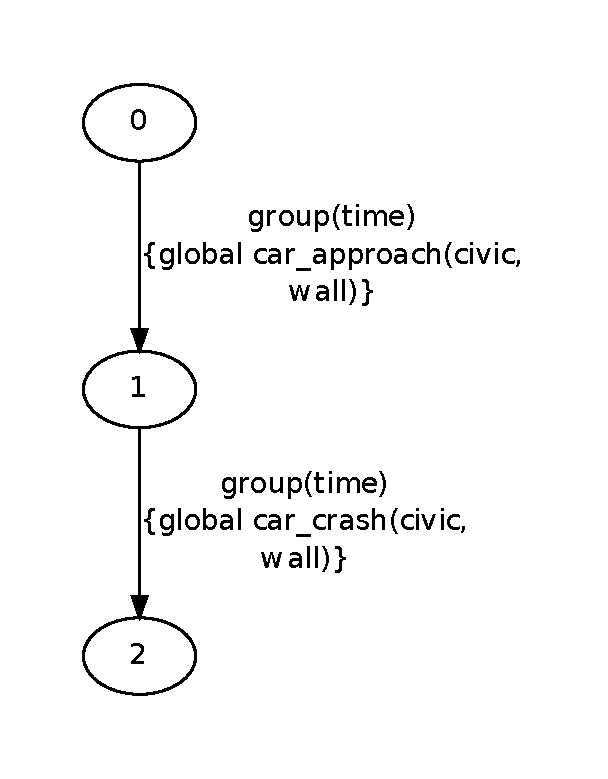
\includegraphics[height=3in]{ag_car/simple/full_bunny_1_ag_5}
\caption{Simple car attack graph}
\label{fig:fullbunny_simple_ag}
\end{figure}

Suppose the initial conditions were changed so that the \texttt{compromised}
quality began as \texttt{false}, and an additional exploit called \texttt{own}
were added so as to match the patterns given in Fig.~\ref{fig:fullbunny_one_xp}.

\begin{figure}
\begin{lstlisting}
global group(time) exploit car_depart(c,w)=
    preconditions:
        platform:c,cpe:/h:honda;
        quality:c,compromised != true;
        platform:w,cpe:/h::wall;
        quality:c,status=up;
    postconditions:
        update topology:c<->w,distance+=25;
.

global group(time) exploit car_approach(c,w)=
    preconditions:
        platform:c,cpe:/h:honda;
        quality:c,compromised=true;
        platform:w,cpe:/h::wall;
        quality:c,status=up;
        topology:c<->w,distance>25;
    postconditions:
        update topology:c<->w,distance-=25;
.

global group(time) exploit car_crash(c,w)=
    preconditions:
        platform:c,cpe:/h:honda;
        quality:c,compromised=true;
        platform:w,cpe:/h::wall;
        quality:c,status=up;
        topology:c<->w,distance<=25;
    postconditions:
        update topology:c<->w,distance:=0;
        update quality:c,status=down;
.

exploit own_civic(c)=
    preconditions:
        platform:c,cpe:/h:honda:civic;
        quality:c,compromised=false;
        quality:c,status=up;
    postconditions:
        update quality:c,compromised=true;
.
\end{lstlisting}
\caption{One-car hybrid example}
\label{fig:fullbunny_one_xp}
\end{figure}

In this case, the resulting attack graph (shown in 
Fig.~\ref{fig:fullbunny_one_ag} to a maximum generation depth of 5) clearly
illustrates the interaction of the discrete behavior of the attacker (an
attack occuring in the ``cyber'' world) with the continuous evolution of the
car (in the physical world). This embodies a common trait of hybrid systems
and also hybrid attacks: their discrete behavior acts to place them into
operational modes wherein the passage of time causes important behavior. In
this case, the evolution of time is clearly denoted by the transitions labeled
\texttt{group(time)}.

\begin{figure}
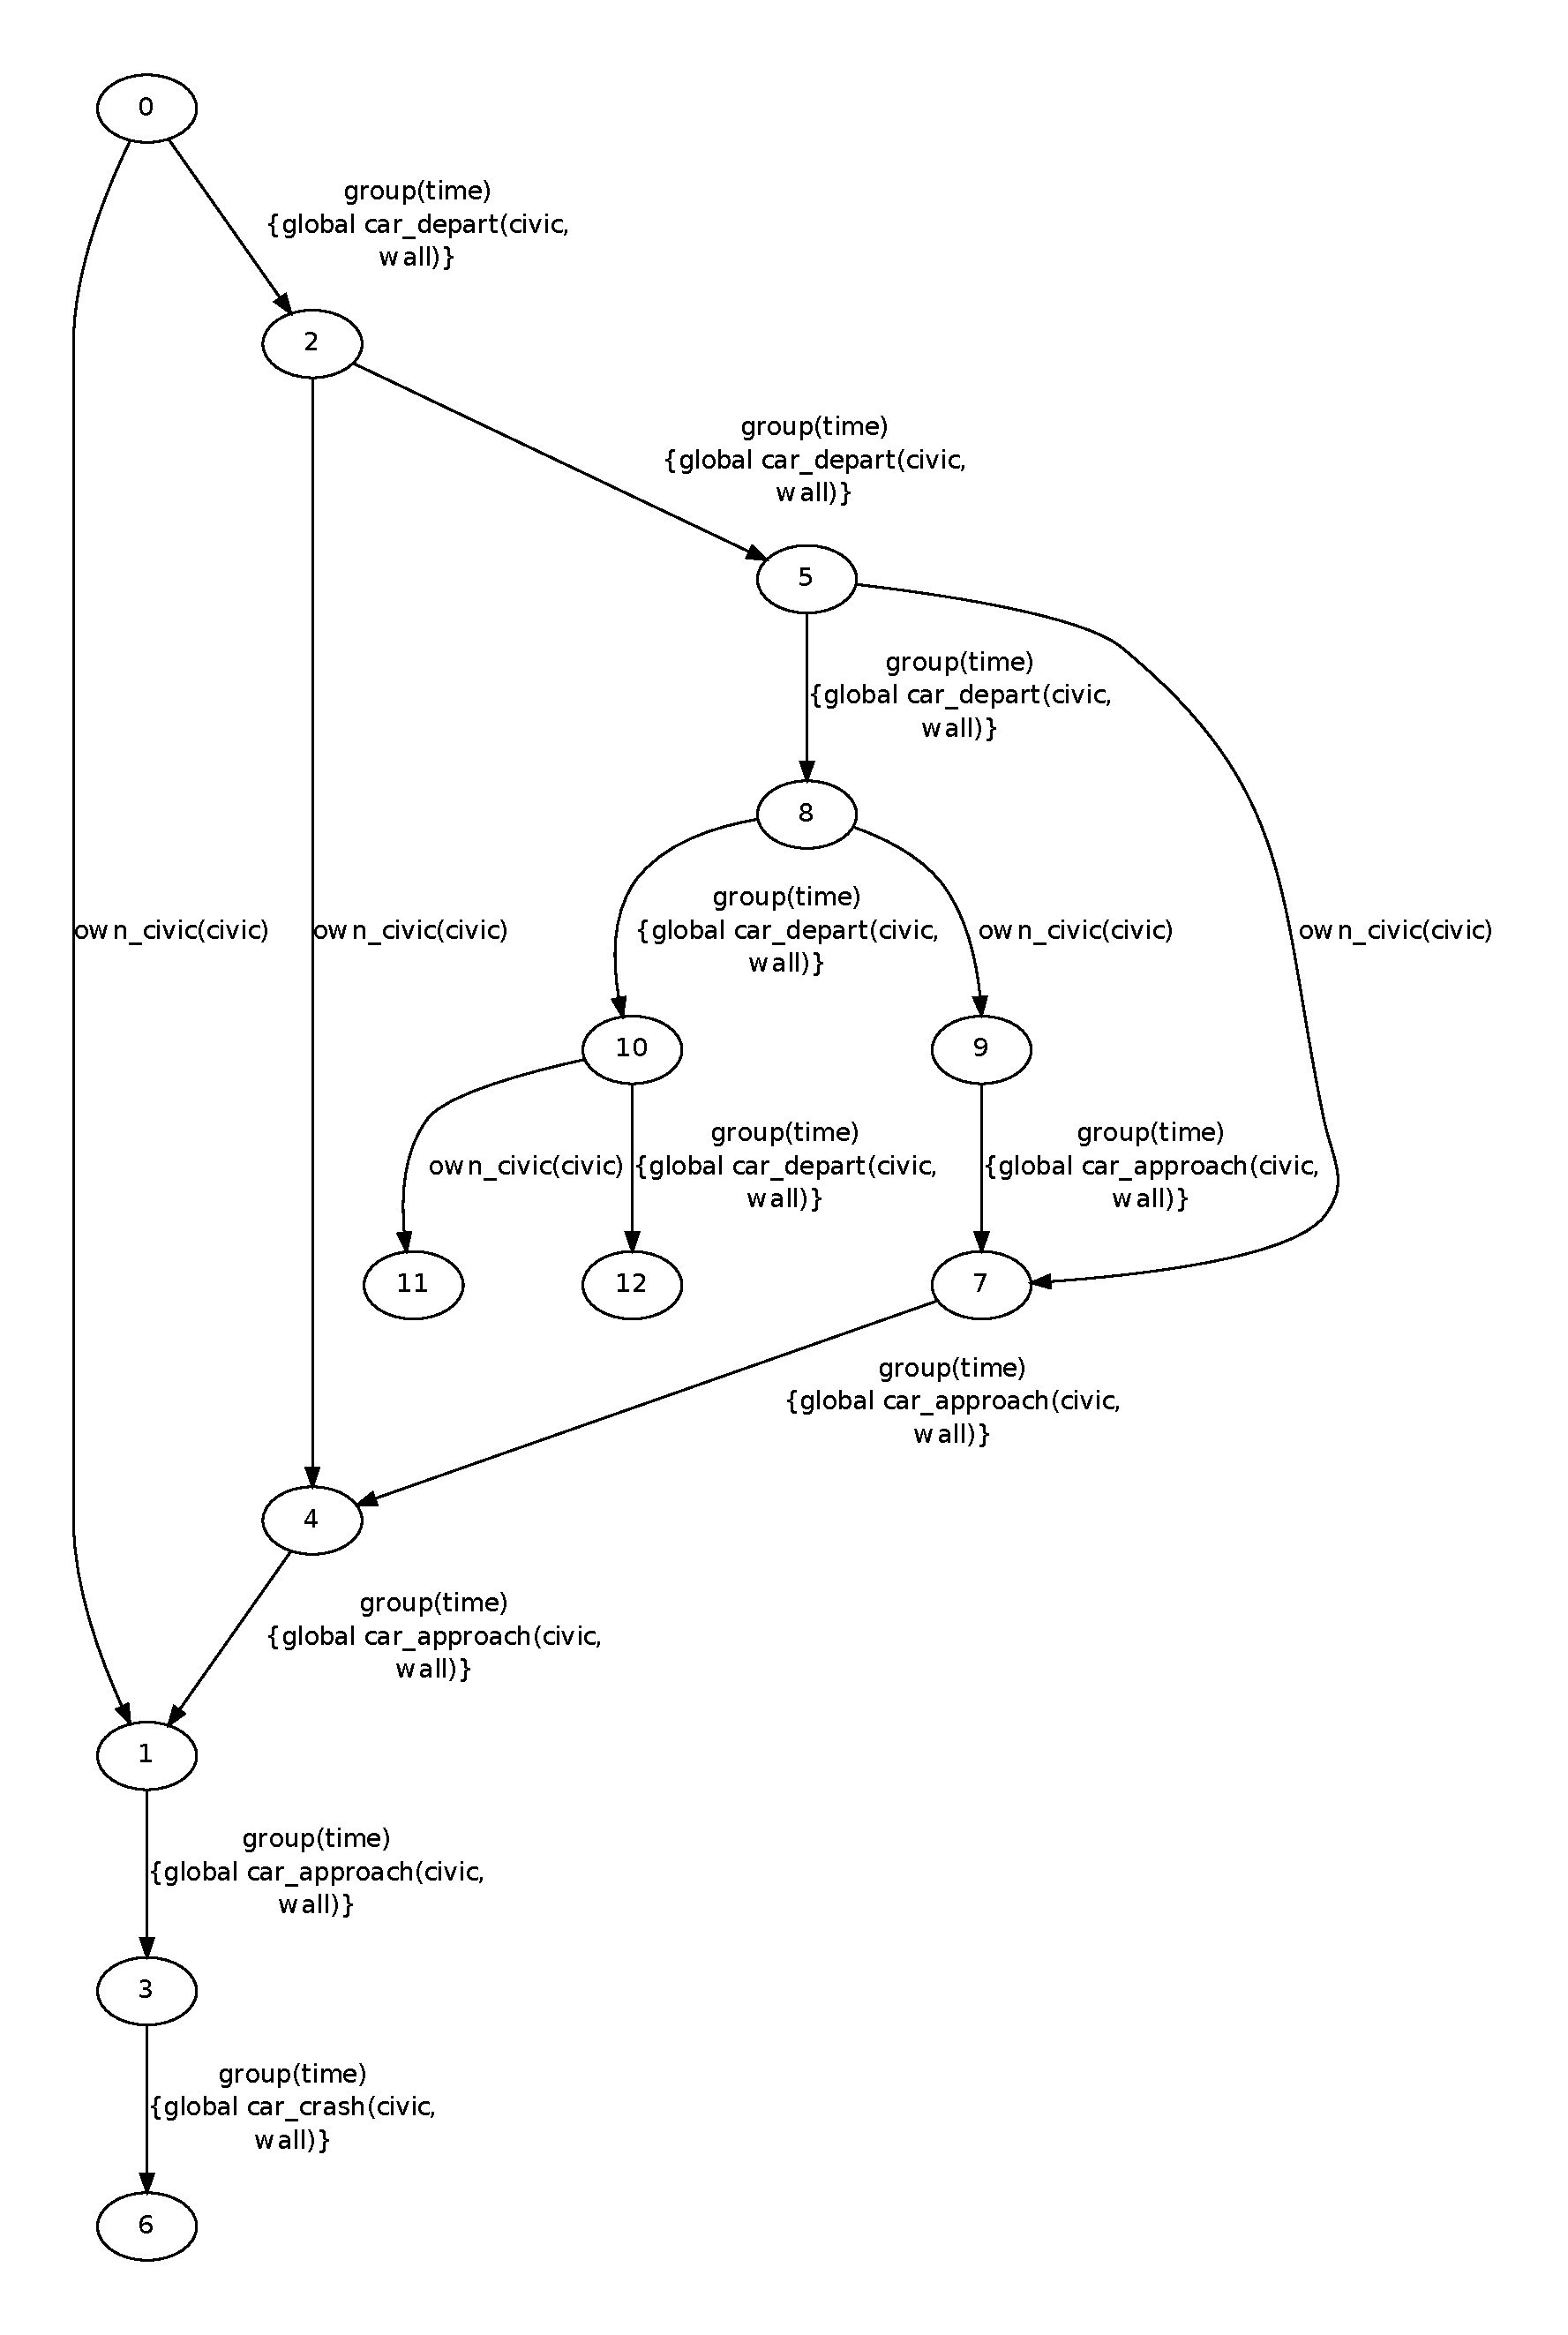
\includegraphics[width=6in]{ag_car/onecar/full_bunny_onecar_ag_5}
\caption{One-car automotive attack graph}
\label{fig:fullbunny_one_ag}
\end{figure}

One final automobile example serves to illustrate the behavior of the
combined global and grouped exploits and their use in implementing
timing behavior. Consider the case in which, while the exploits remain
as in the previous example's definition in Fig.~\ref{fig:fullbunny_one_xp},
an additional nearby car is introduced that seeks to drive away from the wall
at the same rate as \texttt{civic} but that is \emph{not} vulnerable to the 
discrete \texttt{own} exploit. This network model is provided in 
Fig.~\ref{fig:fullbunny_two_nm}.

\begin{figure}
\begin{lstlisting}
network model=
    assets:
        civic;
        accord;
        wall;
    facts:
        platform:civic,cpe:/h:honda:civic;
        quality:civic,compromised=false;
        quality:civic,status=up;
        
        platform:accord,cpe:/h:honda:accord;
        quality:accord,compromised=false;
        quality:accord,status=up;

        platform:wall,cpe:/h::wall;

        topology:civic<->wall,distance:=50;
        topology:accord<->wall,distance:=60;
.
\end{lstlisting}
\caption{Two-car example network model}
\label{fig:fullbunny_two_nm}
\end{figure}

The resulting attack graph is provided in Fig.~\ref{fig:fullbunny_two_ag}.
Observe the sometimes heterogeneity of the time evolution exploit groups.
Of particular interest is the transition from state 3 to state 6, in which
the crashing of the Civic has the discrete consequence of placing it into a
mode in which it no longer changes state with time.

\begin{figure}
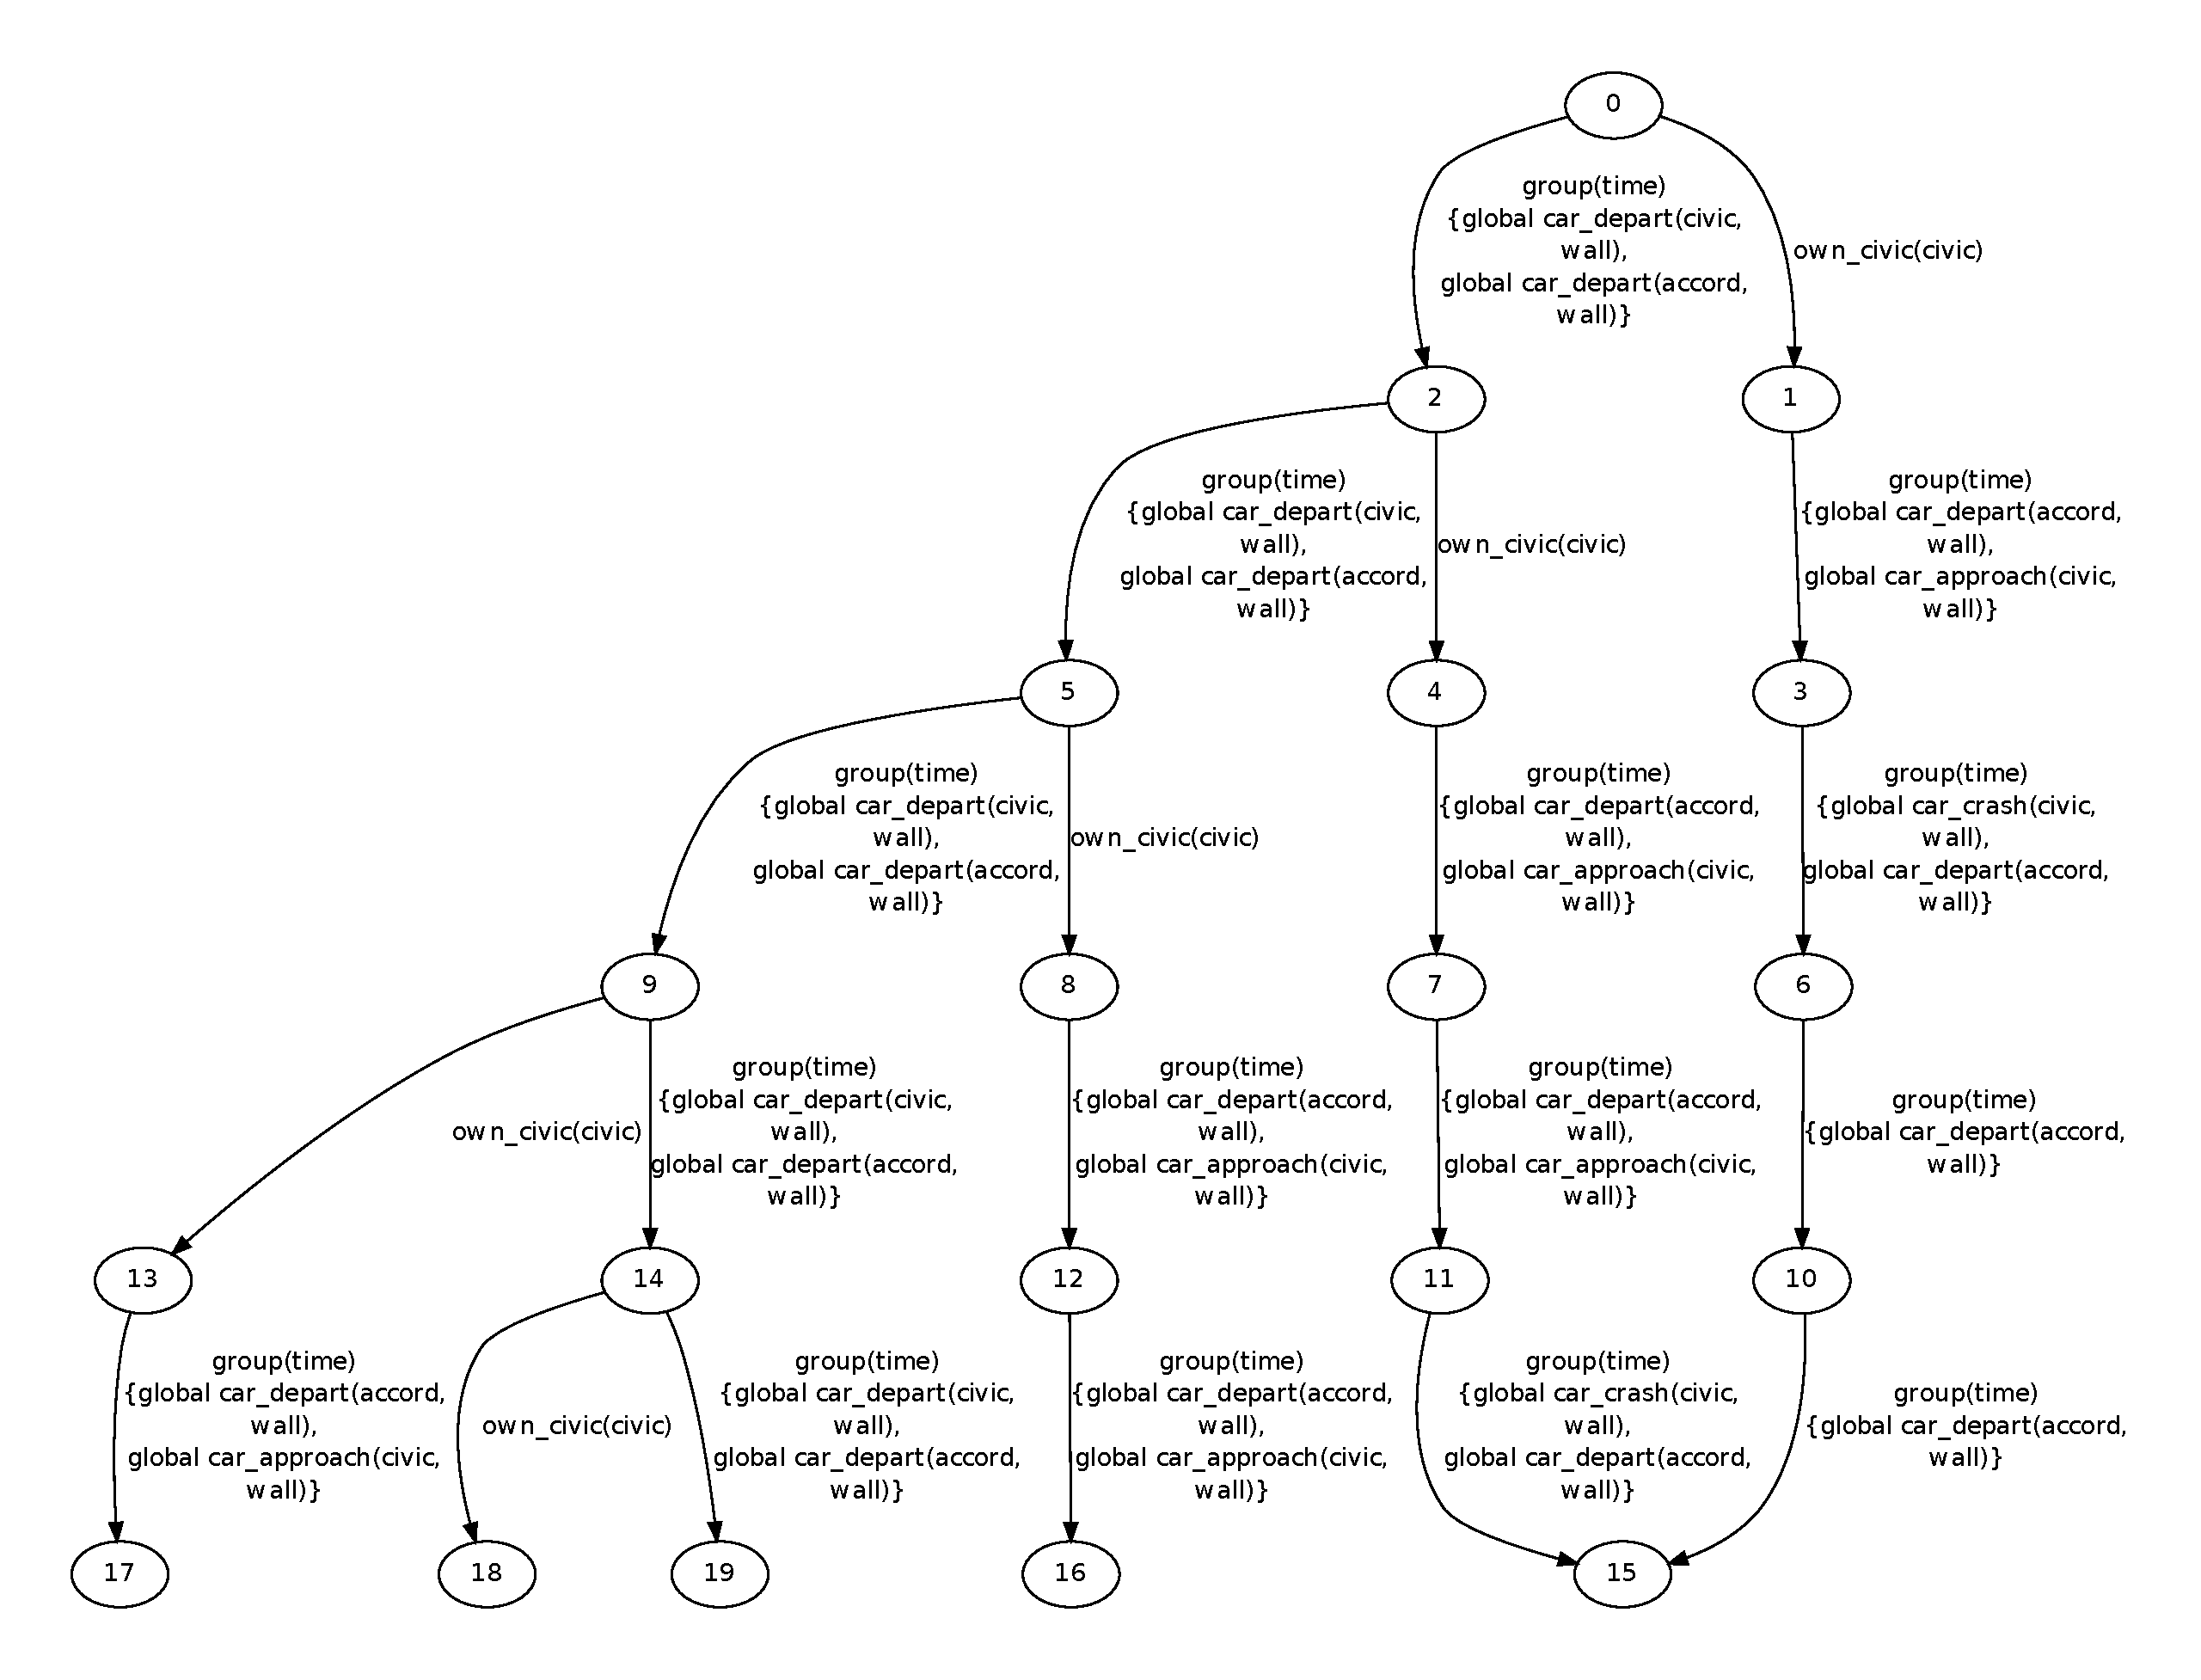
\includegraphics[width=6in]{ag_car/twocar/full_bunny_twocar_ag_5}
\caption{Two-car automotive attack graph}
\label{fig:fullbunny_two_ag}
\end{figure}
\TUsubsection{Denial of Sleep}
The final example serves to demonstrate further the interaction of discrete
attacks with time; it is also used later to discuss scaling behavior. The network
model given in Fig.~\ref{fig:rfid1_nm} describes a system of a single
RFID reader with a single RFID tag, in the ISO 18000-7 system as described 
in section~\ref{sec:bg:rfid}. The tag begins with a battery life of 100, which
is drained at a rate of 25 per time step if the sleep denial attack is being
executed, and at a rate of 10 per time step if not. This behavior is shown in
the exploit patterns in Fig.~\ref{fig:rfid1_xp2}, along with
the discrete attacks \texttt{own\_reader} (which gives the attacker control of
the reader) and \texttt{deny\_sleep} (which causes a tag to enter the
denial of sleep mode) in Fig.~\ref{fig:rfid1_xp1}.

\begin{figure}
\begin{lstlisting}
network model = 
    assets :
        attacker;
        reader;
        tag0;
    
    facts :
        # Reader:
        platform:reader,cpe:/h::VulnerableReader;
        quality:reader,status=up;
        
        # Tag:
        platform:tag0,cpe:/h::Tag;
        quality:tag0,status=up;
        quality:tag0,power:=100;
        quality:tag0,mode=sleep;
        
        # Topologies:
        topology:attacker -> reader,connected_network;
        topology:reader -> tag0,connected_rfid;
.
\end{lstlisting}
\caption{One tag RFID system network model}
\label{fig:rfid1_nm}
\end{figure}

\begin{figure}
\begin{lstlisting}
exploit own_reader(a, r)=
    preconditions:
        platform:r,cpe:/h::VulnerableReader;
        quality:r,status=up;
        topology:a->r,connected_network;
    postconditions:
        insert topology:a->r,access_admin;
.

exploit deny_sleep(a, r, t)=
    preconditions:
        platform:r,cpe:/h::VulnerableReader;
        quality:r,status=up;
        
        platform:t,cpe:/h::Tag;
        quality:t,status=up;
        quality:t,mode=sleep;
        
        topology:a->r,access_admin;
        topology:r->t,connected_rfid;
    postconditions:
        update quality:t,mode=wake;
.
\end{lstlisting}
\caption{One tag RFID system discrete exploit patterns}
\label{fig:rfid1_xp1}
\end{figure}



\begin{figure}
\begin{lstlisting}
global group(time) exploit wake_power_dec(t)=
    preconditions:
        platform:t,cpe:/h::Tag;
        quality:t,status=up;
        quality:t,mode=wake;
        quality:t,power>25;
    postconditions:
        update quality:t,power-=25;
.

global group(time) exploit sleep_power_dec(t)=
    preconditions:
        platform:t,cpe:/h::Tag;
        quality:t,mode=sleep;
        quality:t,status=up;
        quality:t,power>10;
    postconditions:
        update quality:t,power-=10;
.

global group(time) exploit wake_power_die(t)=
    preconditions:
        platform:t,cpe:/h::Tag;
        quality:t,mode=wake;
        quality:t,status=up;
        quality:t,power<=25;
    postconditions:
        update quality:t,power:=0;
        update quality:t,status=down;
.

global group(time) exploit sleep_power_die(t)=
    preconditions:
        platform:t,cpe:/h::Tag;
        quality:t,mode=sleep;
        quality:t,status=up;
        quality:t,power<=10;
    postconditions:
        update quality:t,power:=0;
        update quality:t,status=down;
.
\end{lstlisting}
\caption{One tag RFID system continuous exploit patterns}
\label{fig:rfid1_xp2}
\end{figure}

Two attack graphs help to demonstrate the execution of this model. The first is
given in Fig.~\ref{fig:rfid1_ag6}, which is the attack graph generated to a
depth of 6. Observe that the leftmost set of edges is the worst case
scenario: the attacker immediately takes control of the network and kills
the tags in only 4 timesteps. The rightmost edge, then, is the best case
scenario: in this situation, the attacker never (at least to a generation
depth of 6) acts. The only transitions are those caused by the normal
time evolution of the system.

Likewise, Fig.~\ref{fig:rfid1_ag11} is the attack graph generated to its
full depth. There are only two leaf nodes: state 21, in which the attacker
has executed the denial of sleep attack to the demise of the tag, and state
40, in which the tag has died on its own.

\begin{figure}
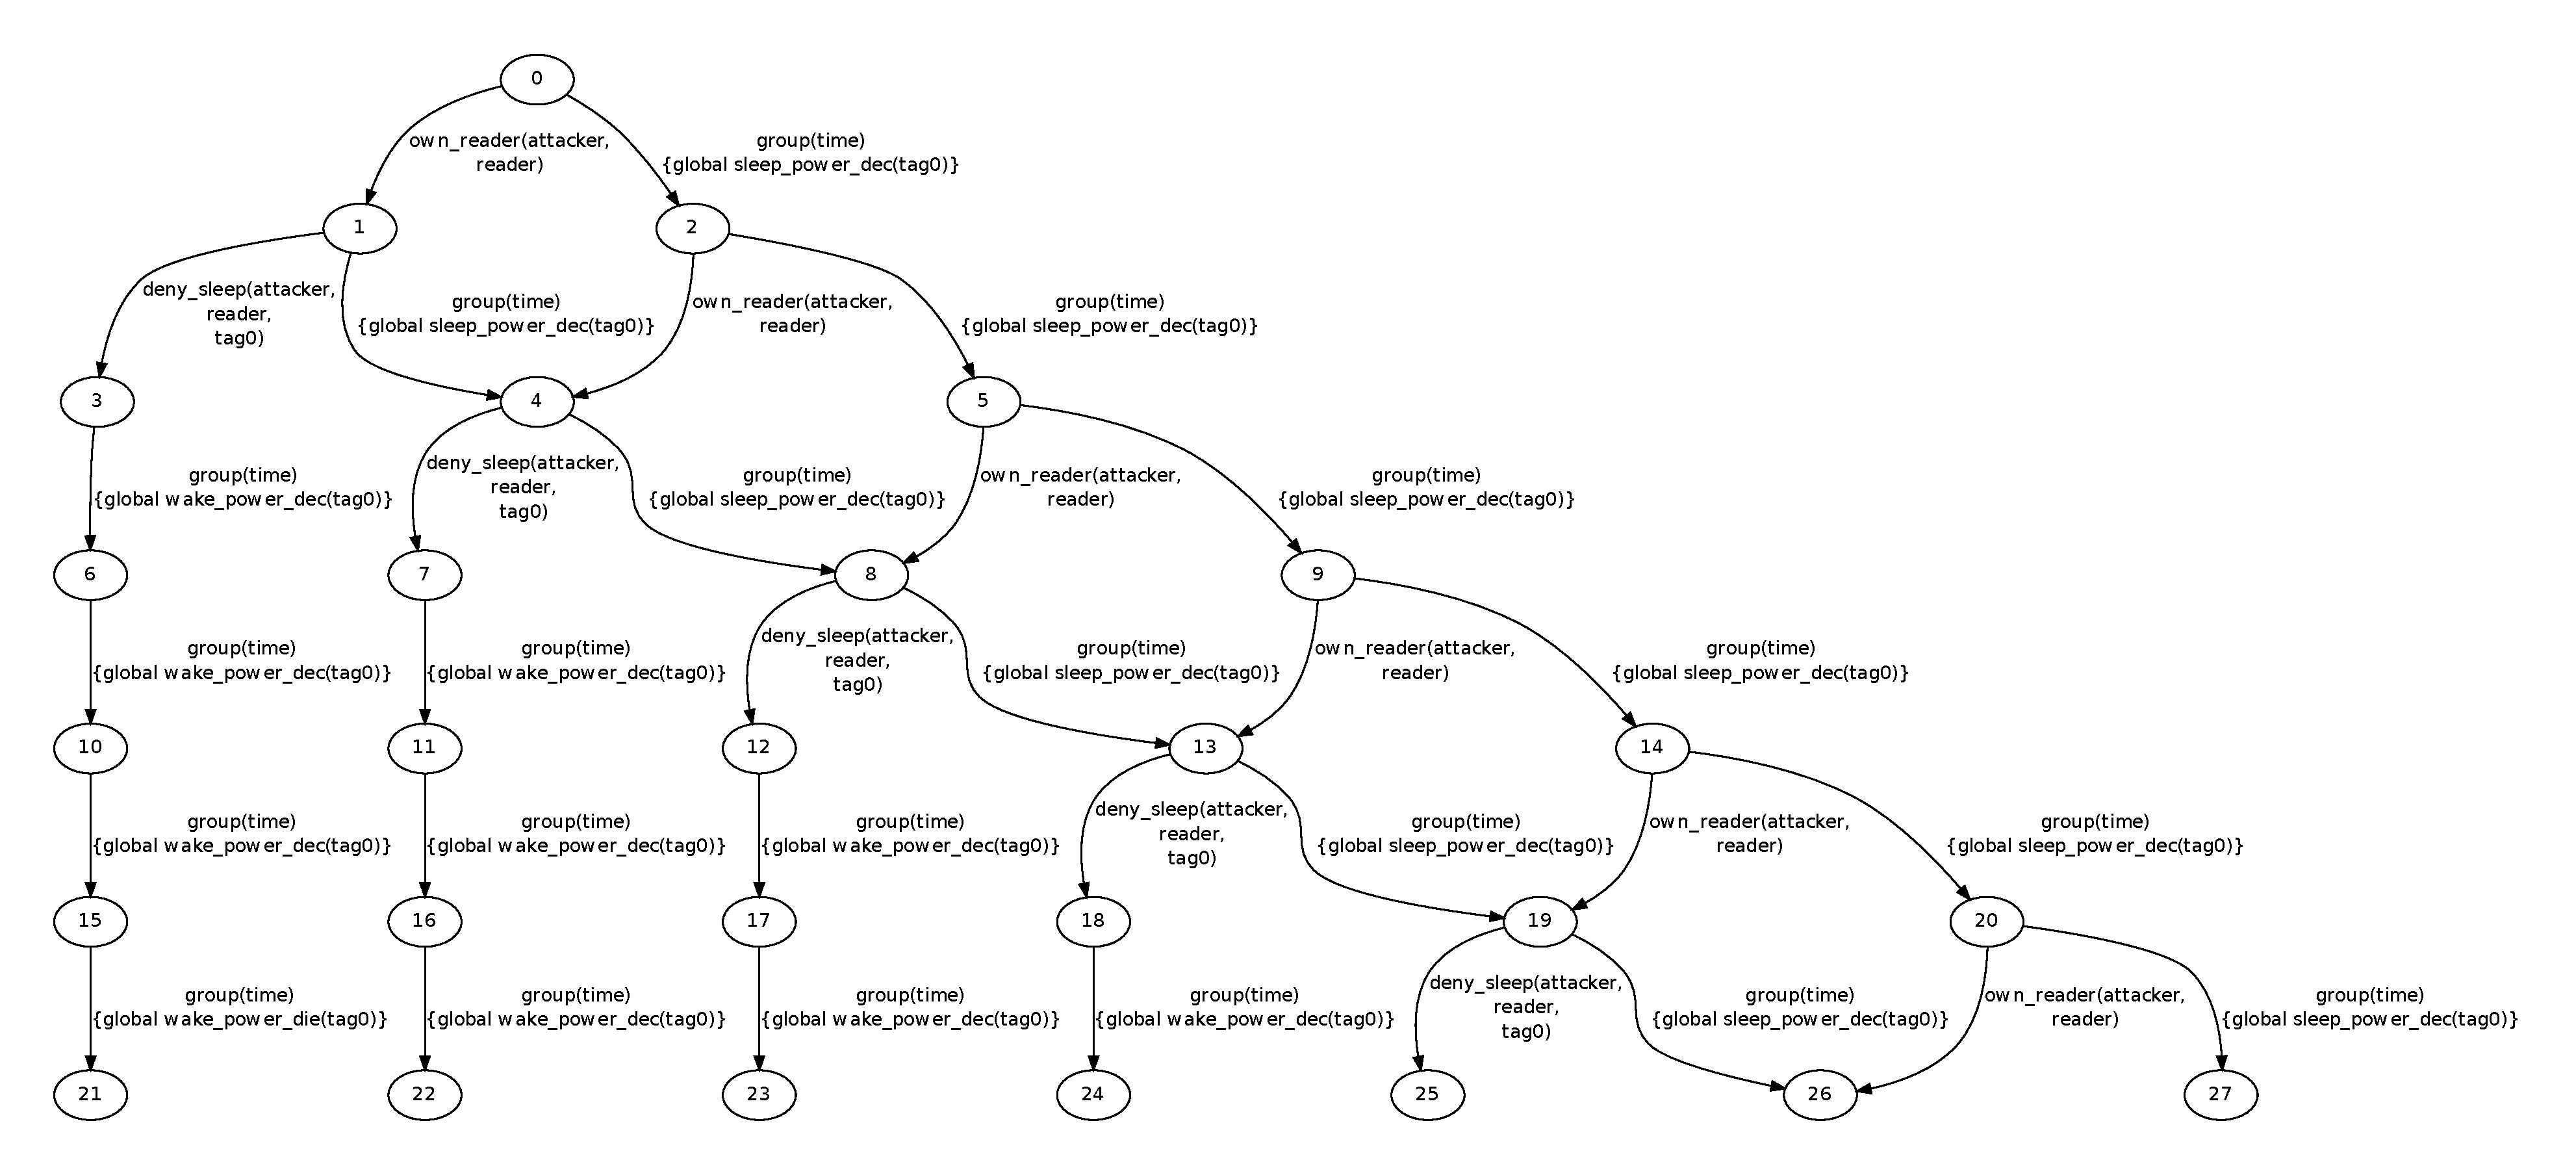
\includegraphics[width=6in]{ag_dash7/sleep_ag_6}
\caption{One tag RFID system attack graph (depth of 6)}
\label{fig:rfid1_ag6}
\end{figure}

\begin{figure}
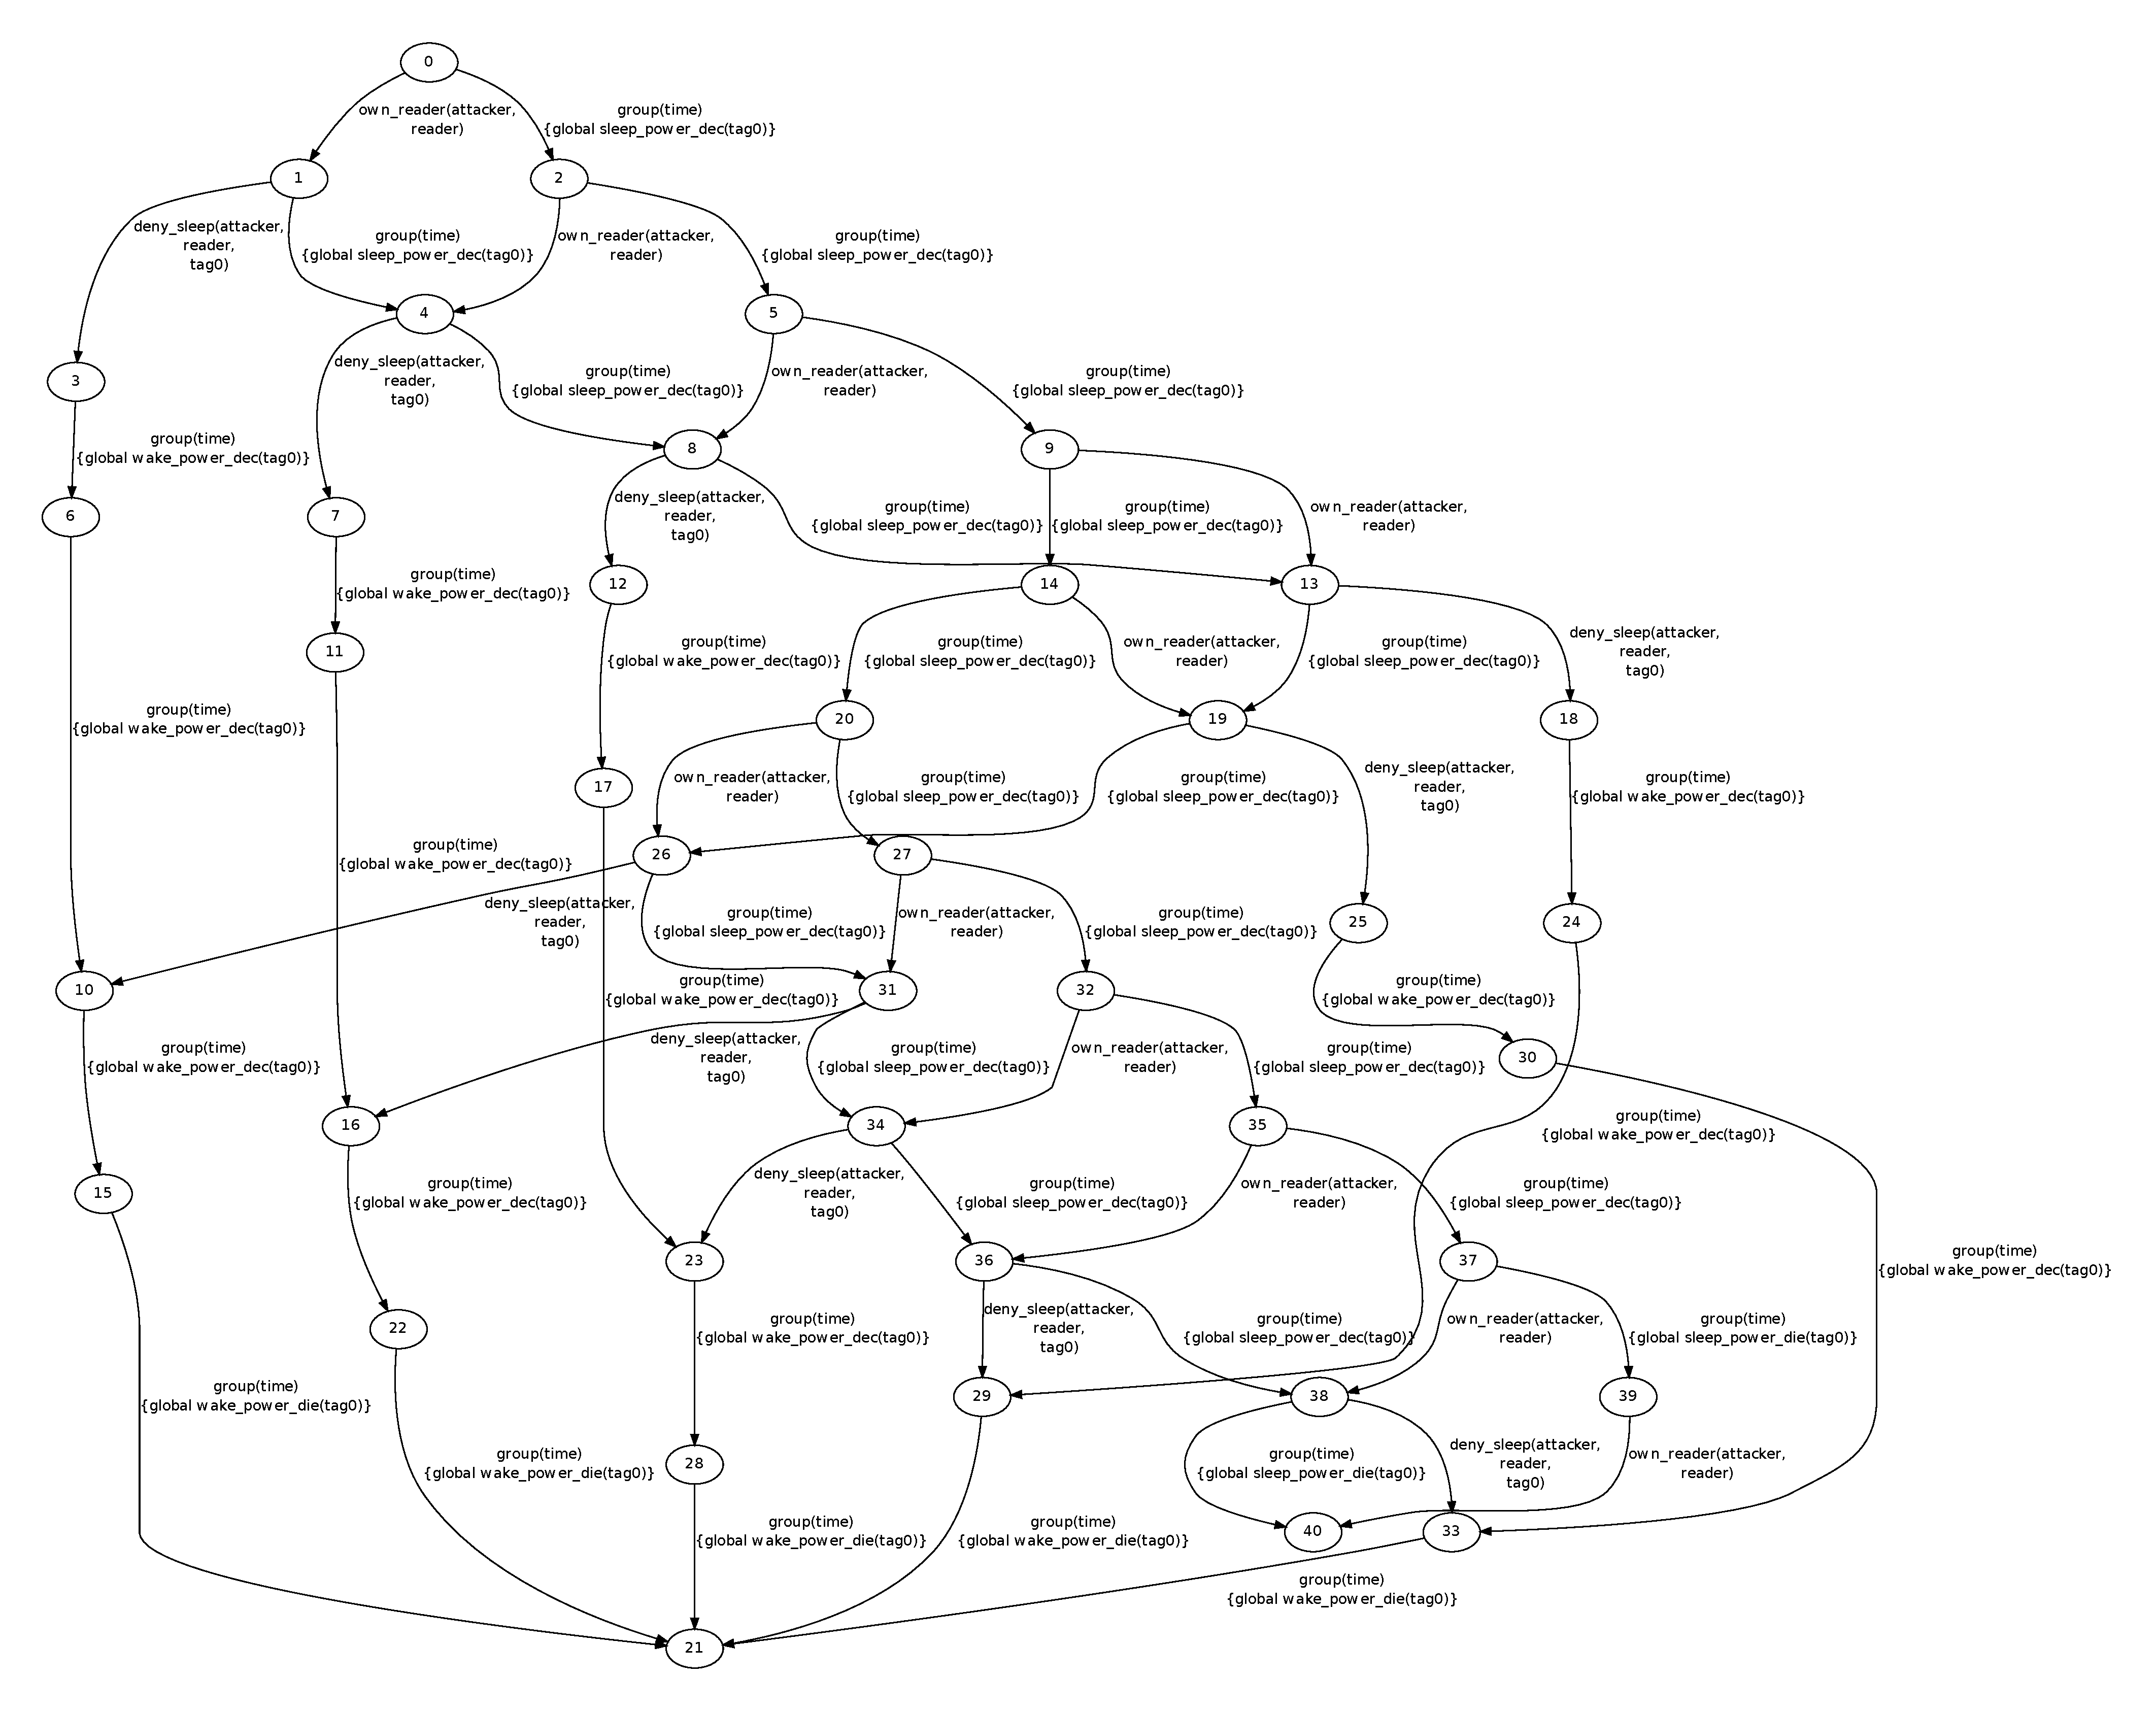
\includegraphics[width=6in]{ag_dash7/sleep_ag_11}
\caption{One tag RFID system attack graph (full depth)}
\label{fig:rfid1_ag11}
\end{figure}
\TUchapter{Conclusion and Future Work}

% Hybrid first and third person strategy -- local and adjacent access 
% are topologies; network connection is a quality and therefore assumed
% topology.

% STRIDE integration

% regex/wildcard exploits

%%%%%%%%%%%%%%%%%%%%%%%%%%%%%%%%%
% BIBLIOGRAPHY
%%%%%%%%%%%%%%%%%%%%%%%%%%%%%%%%%

%\addtocontents{toc}{\protect{\hfill \ }}
%\addcontentsline{toc}{section}{\contentsadj NOMENCLATURE}

\bibliographyp
\bibliography{TUthesis}
\bibliographystyle{plain}

%%%%%%%%%%%%%%%%%%%%%%%%%%%%%%%%%
% APPENDICES AS NECESSARY
%%%%%%%%%%%%%%%%%%%%%%%%%%%%%%%%%

\appendixpages       % prepare for the generation of the appendices
%\include{Appendices}
\end{document}
